%%%% Author: Lu Niu, lukeniu@outlook.com

%% Document declaration
\documentclass[xcolor=dvipsnames]{beamer}

%% Packages invoking
\usetheme{SimplePlus}
% \usecolortheme{dolphin}
\usecolortheme{dove}
\usefonttheme{serif}
\usepackage{adjustbox}
\usepackage{amsmath}
\usepackage{bm}
\usepackage{booktabs} % Allows the use of \toprule, \midrule and \bottomrule in tables.
\usepackage{graphicx} % Allows including images.
\usepackage{helvet}
\usepackage{hyperref}
\usepackage{lmodern}
\usepackage{tikz}
\usepackage{xcolor}
\usetikzlibrary{fit, shadows}

%% Fundamental settings
% % Colors (default)
% \definecolor{midTheme}{HTML}{6482E6}          % #6482E6
% \definecolor{shallowTheme}{HTML}{78A0FF}      % #78A0FF
% \definecolor{lightTheme}{HTML}{96B4FF}        % #96B4FF
% Colors (USyd)
\definecolor{midTheme}{HTML}{E64628}            % #E64628
\definecolor{shallowTheme}{HTML}{F07850}        % #F07850
\definecolor{lightTheme}{HTML}{FFA064}          % #FFA064
% Content colors
\definecolor{table1}{HTML}{BBE6DC}              % #BBE6DC
\definecolor{table2}{HTML}{F0FAF5}              % #F0FAF5
\definecolor{table3}{HTML}{E6F5EB}              % #E6F5EB
\definecolor{darkBlue}{HTML}{285FB4}            % #285FB4

% Personal information
\newcommand{\myName}{Lu Niu}
\newcommand{\myDepartment}{School of Phsics}
\newcommand{\myInstitution}{University of Sydney}
\newcommand{\myEmail}{lukeniu@outlook.com}
\newcommand{\progressBarShift}{-2pt}
\newcommand{\placeLogo}{
\begin{tikzpicture}[overlay,remember picture]
    \node[anchor=north west]at(current page.north west){
\includegraphics[width=100pt]{Logo/USydLogo_White.png}};
\end{tikzpicture}
}

%% Progress bar
\makeatletter
\addtobeamertemplate{footline}{
  \color{lightTheme}
  \raisebox{-6pt}{\rlap{\rule{\dimexpr\beamer@startpageofframe\dimexpr\beamer@rightmargin+\textwidth\relax/\beamer@endpageofdocument}{2pt}}}
  \vspace{-2pt}
}
\makeatother

%% Page settings
\setbeamertemplate{frametitle}{
  \begin{tikzpicture}[overlay,remember picture]
    \node[rounded corners, fill=shallowTheme, text=white, text width=\dimexpr\paperwidth-20pt\relax, text depth=-10pt, anchor=north, yshift=-2pt]at(current page.north){
        \fontsize{10}{10}\selectfont\insertframetitle
    };
  \end{tikzpicture}
}
\setbeamertemplate{caption}[numbered]

%%%% Title page information
%% Title
\title[short title]{Graphene-BC Series Bilayers}
\subtitle{Projected electronic density of state}
%% Author information
\author[Lu Niu]{\myName}
\institute[USYD]
{
    \par \href{mailto:\myEmail}{\myEmail}
    \par \vspace*{\baselineskip}
    \par \myDepartment 
    \par \myInstitution
}
\titlegraphic{\placeLogo}
\date{\today}

%%%% Slides
\begin{document}

%% Title page
\begin{frame}
    \begin{tikzpicture}[overlay, remember picture]
        % Background color box
        \node[fill=shallowTheme, rectangle, anchor=north, text width=\paperwidth, minimum height=40pt] at (current page.north) {};
        % Group logo
        \begin{scope}[opacity=0.6]
            \node[anchor=south west, inner sep=8pt, xshift=4pt] at (current page.south west) {
                
\includegraphics[width=48pt]{Logo/USyd_CMT.png}
            };
        \end{scope}
    \end{tikzpicture}
    \vspace*{-10pt}
    \titlepage
\end{frame}

%% Overview and contents: Throughout your presentation, if you choose to use \section{} and \subsection{} commands, these will automatically be printed on this slide as an overview of your presentation.
\begin{frame}{Overview}
    \tableofcontents
\end{frame}

\section{Monolayers}

\subsection{BC\texorpdfstring{$_\text{3}$}{3} (PBE)}
\begin{frame}{\insertsection: \insertsubsection}
\begin{columns}
    \begin{column}{0.5\textwidth}\begin{figure}
        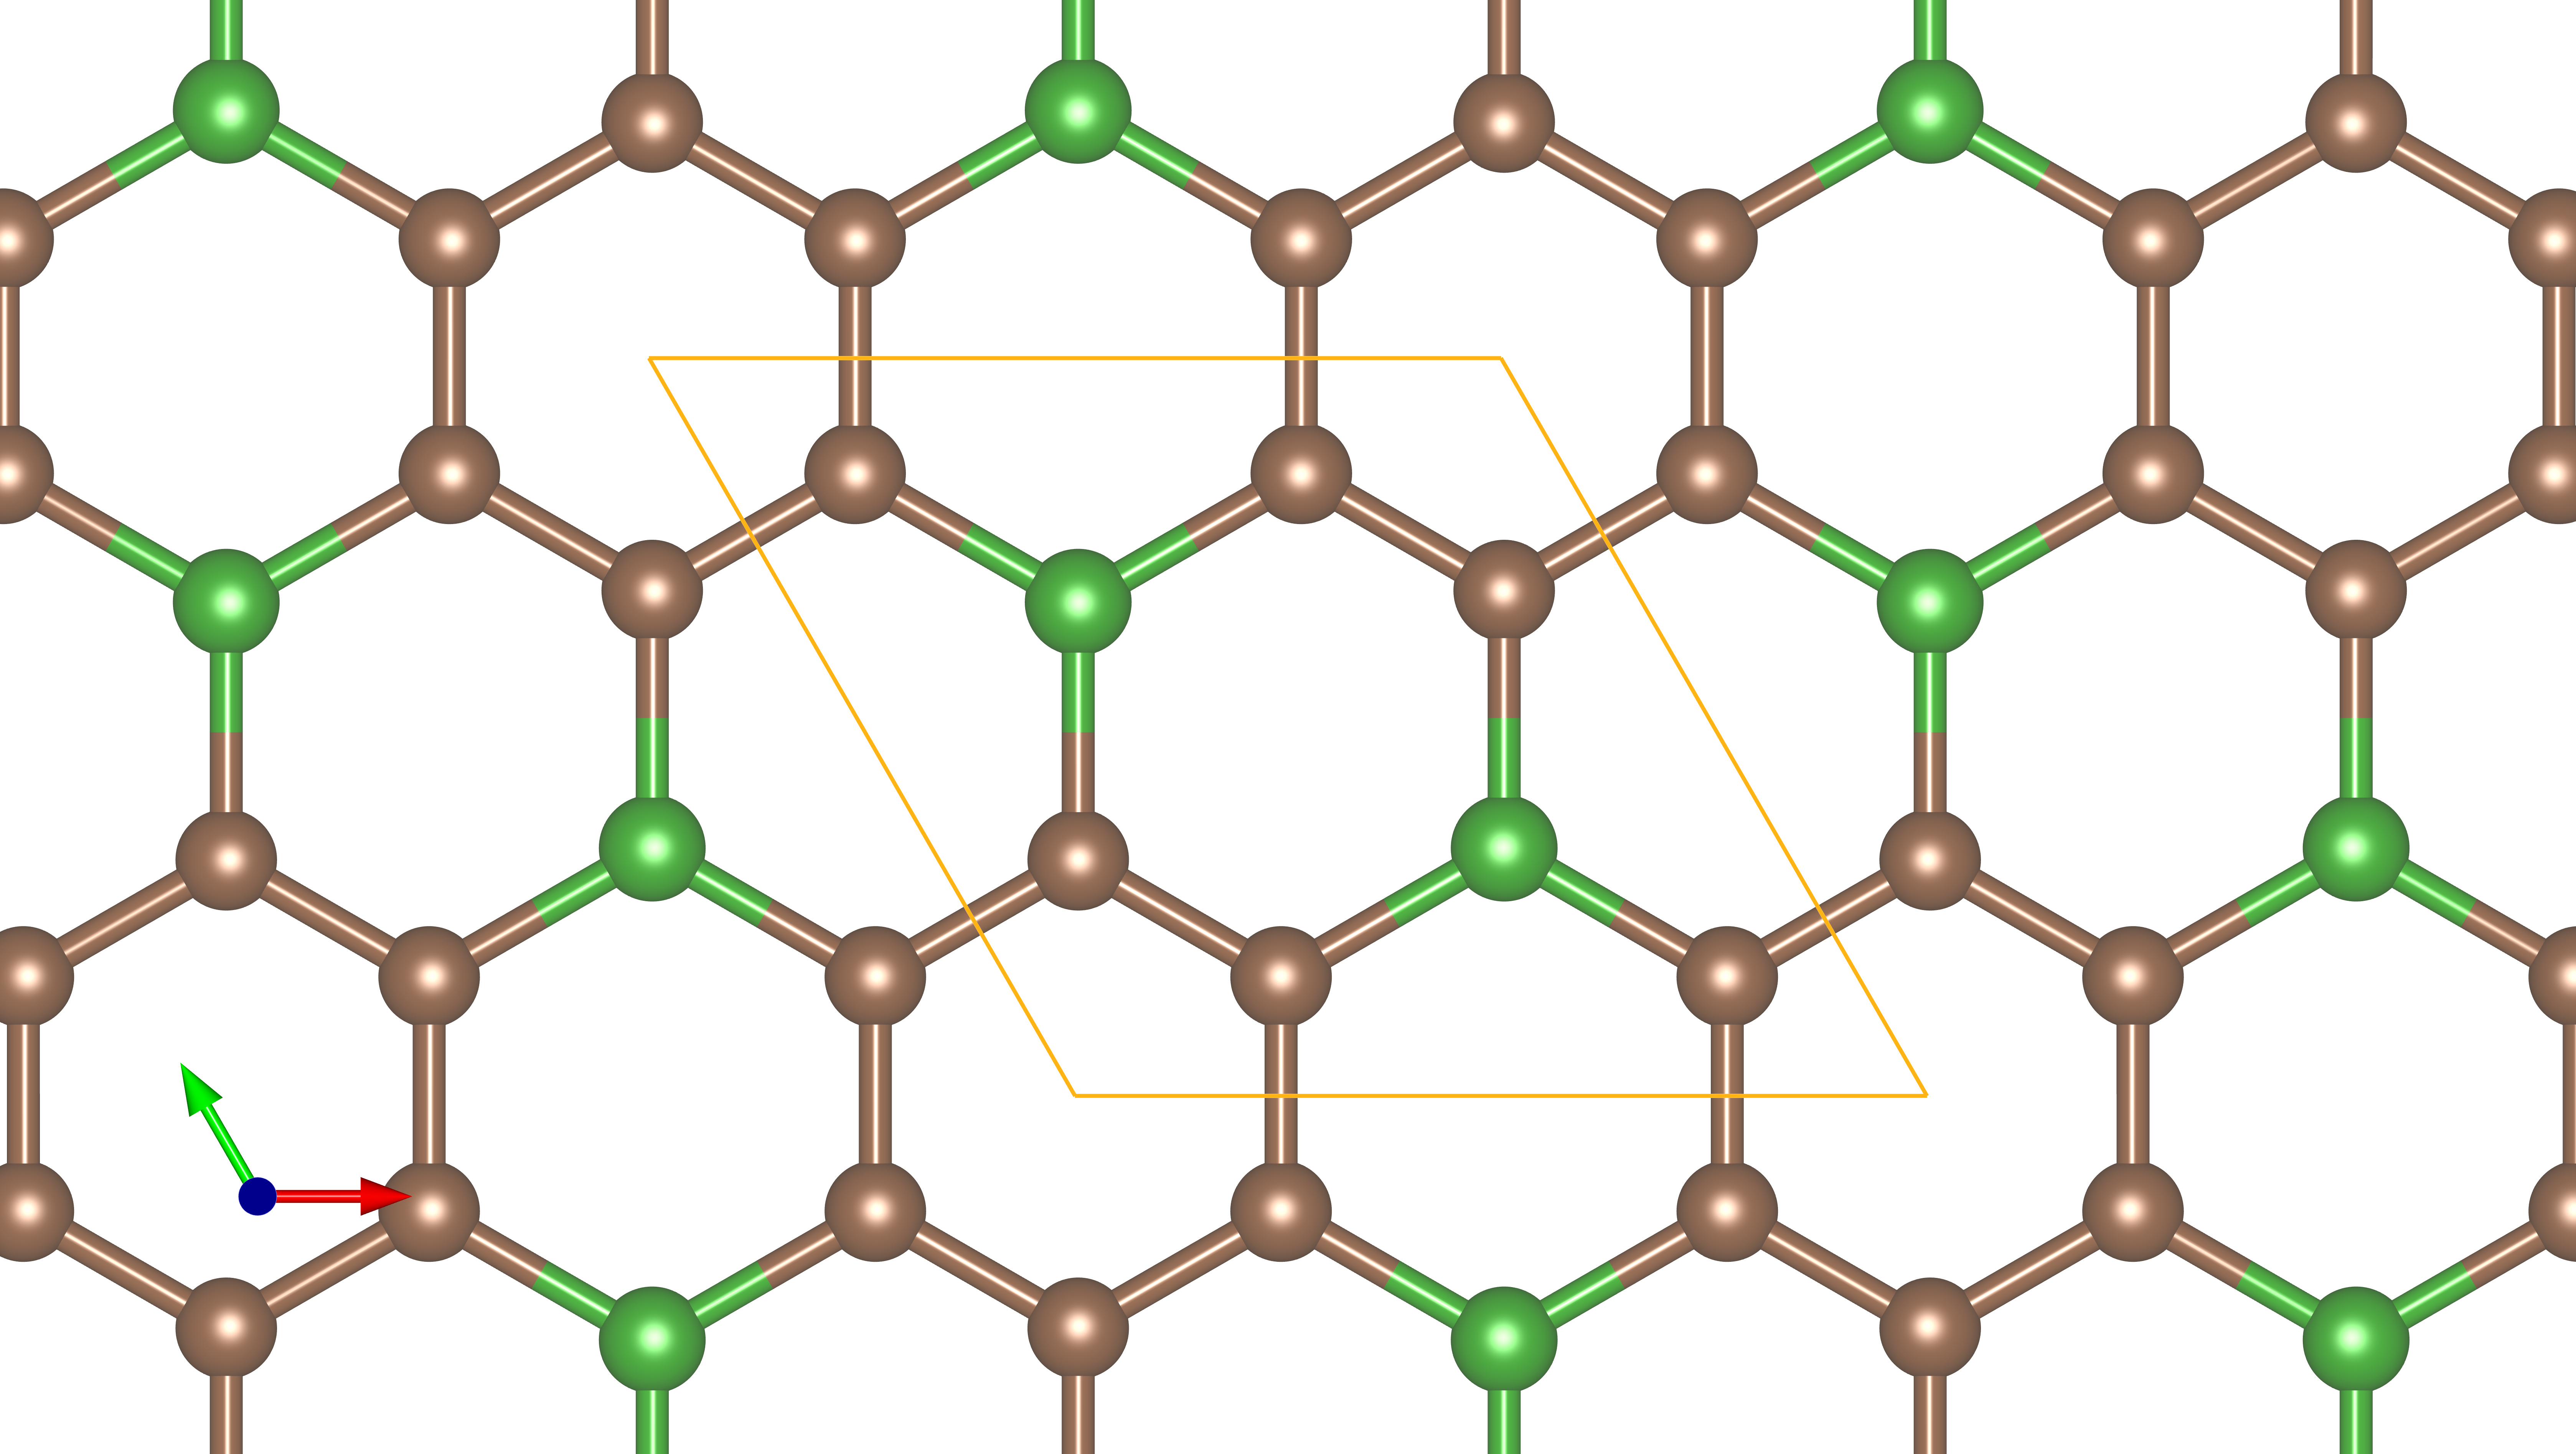
\includegraphics[width=0.5\textwidth]{Supercells/A_BC3.png}
        \caption{BC$_\text{3}$ supercell}
    \end{figure}\end{column}
    \begin{column}{0.5\textwidth}
        \par \textbf{Monolayer: BC$_\text{3}$}
        \par\quad LUMO band: -3.157700;
        \par\quad HOMO band: -3.791800;
        \par\quad Band gap: 0.634100.
    \end{column}
\end{columns}
\begin{columns}
    \begin{column}{0.45\textwidth}\begin{figure}
        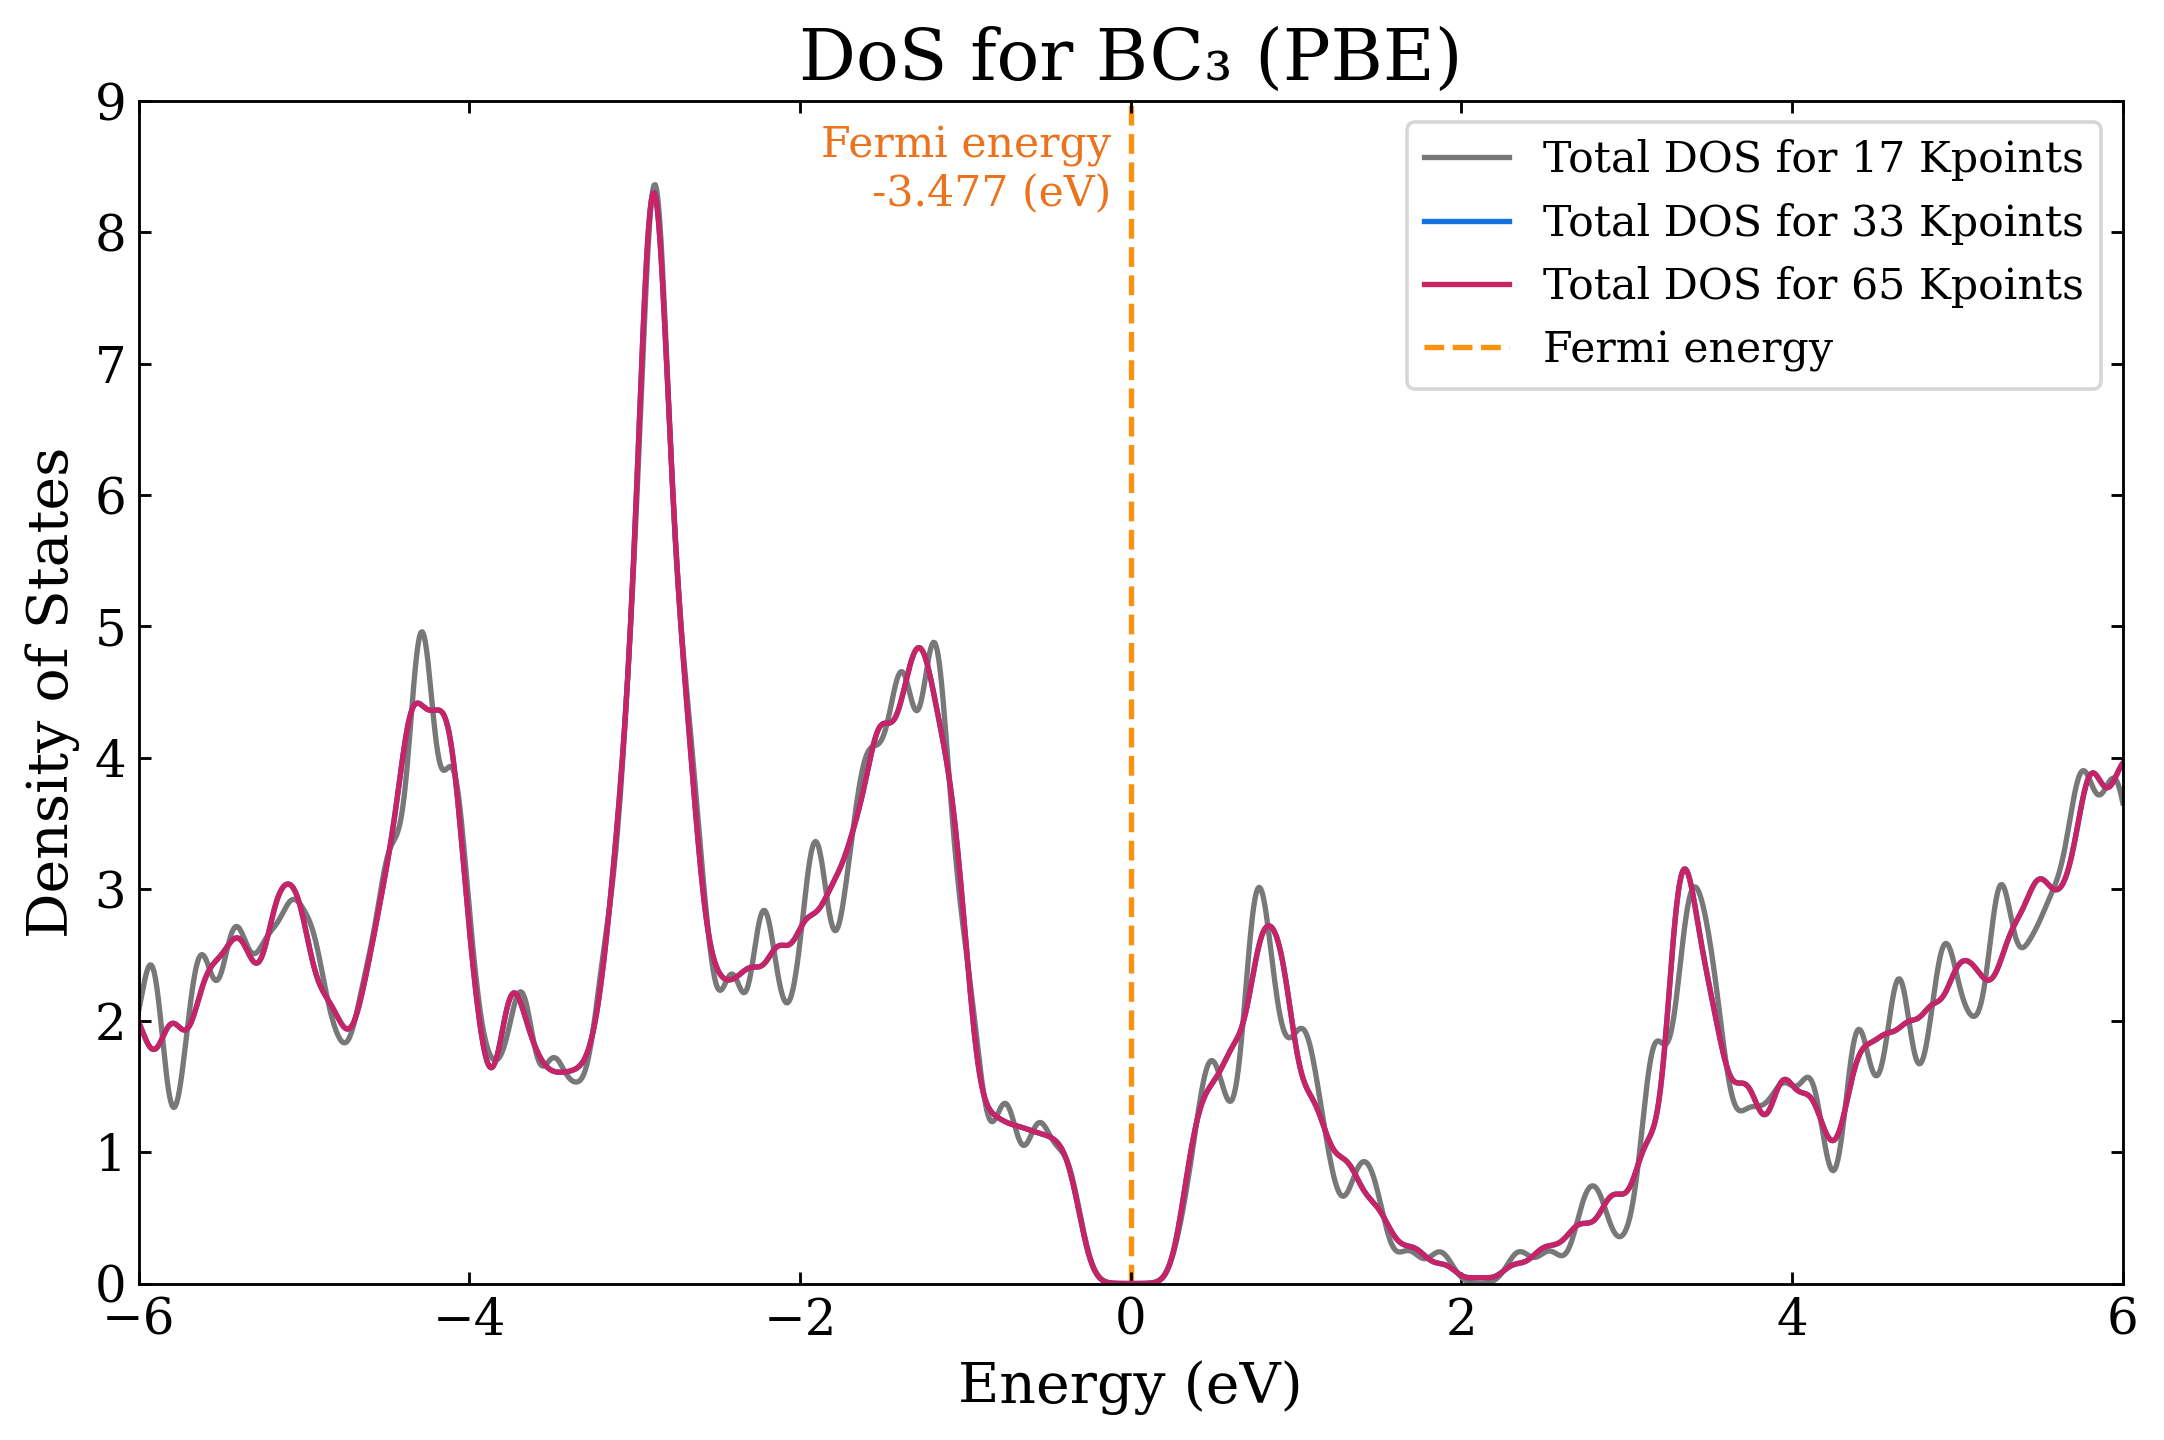
\includegraphics[width=1\textwidth]{PDoS/BC3_dos.png}
        \caption{BC$_\text{3}$ DoS}
    \end{figure}\end{column}
    \begin{column}{0.55\textwidth}\begin{figure}
        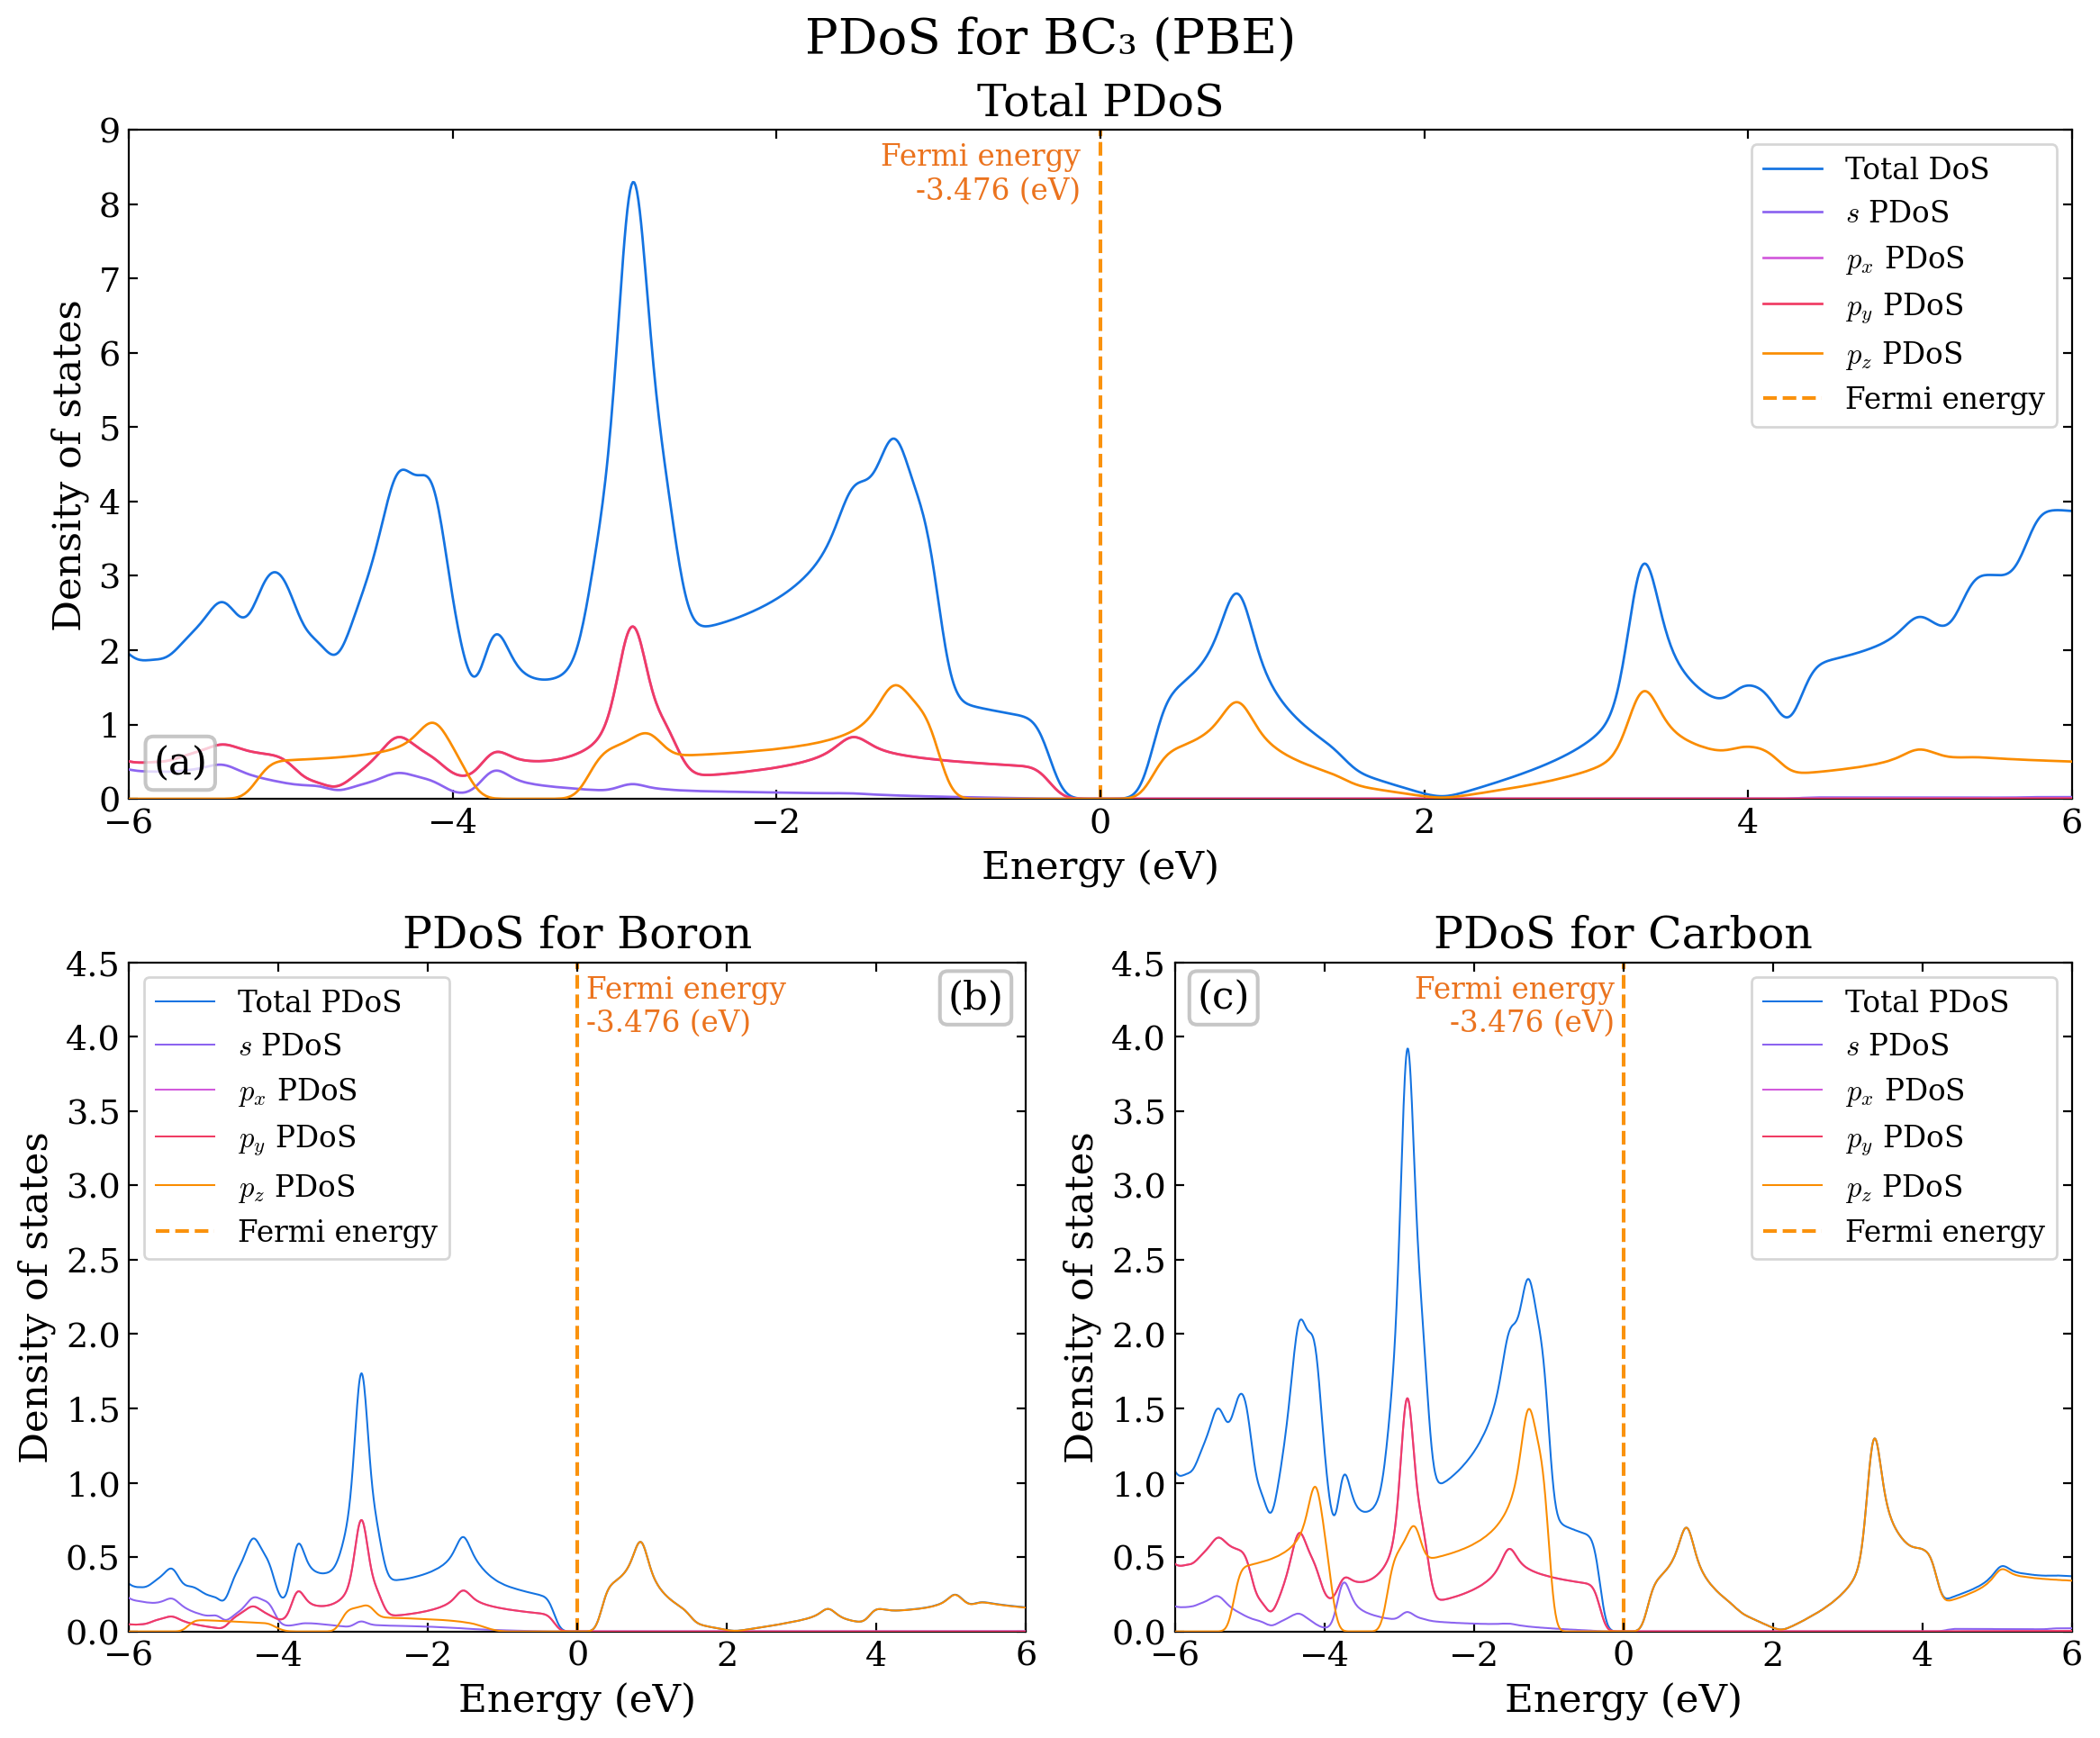
\includegraphics[width=0.8\textwidth]{PDoS/BC3_pdos.png}
        \caption{BC$_\text{3}$ PDoS}
    \end{figure}\end{column}
\end{columns}
\end{frame}

\subsection{Borophene (PBE)}
\begin{frame}{\insertsection: \insertsubsection}
\begin{columns}
    \begin{column}{0.5\textwidth}\begin{figure}
        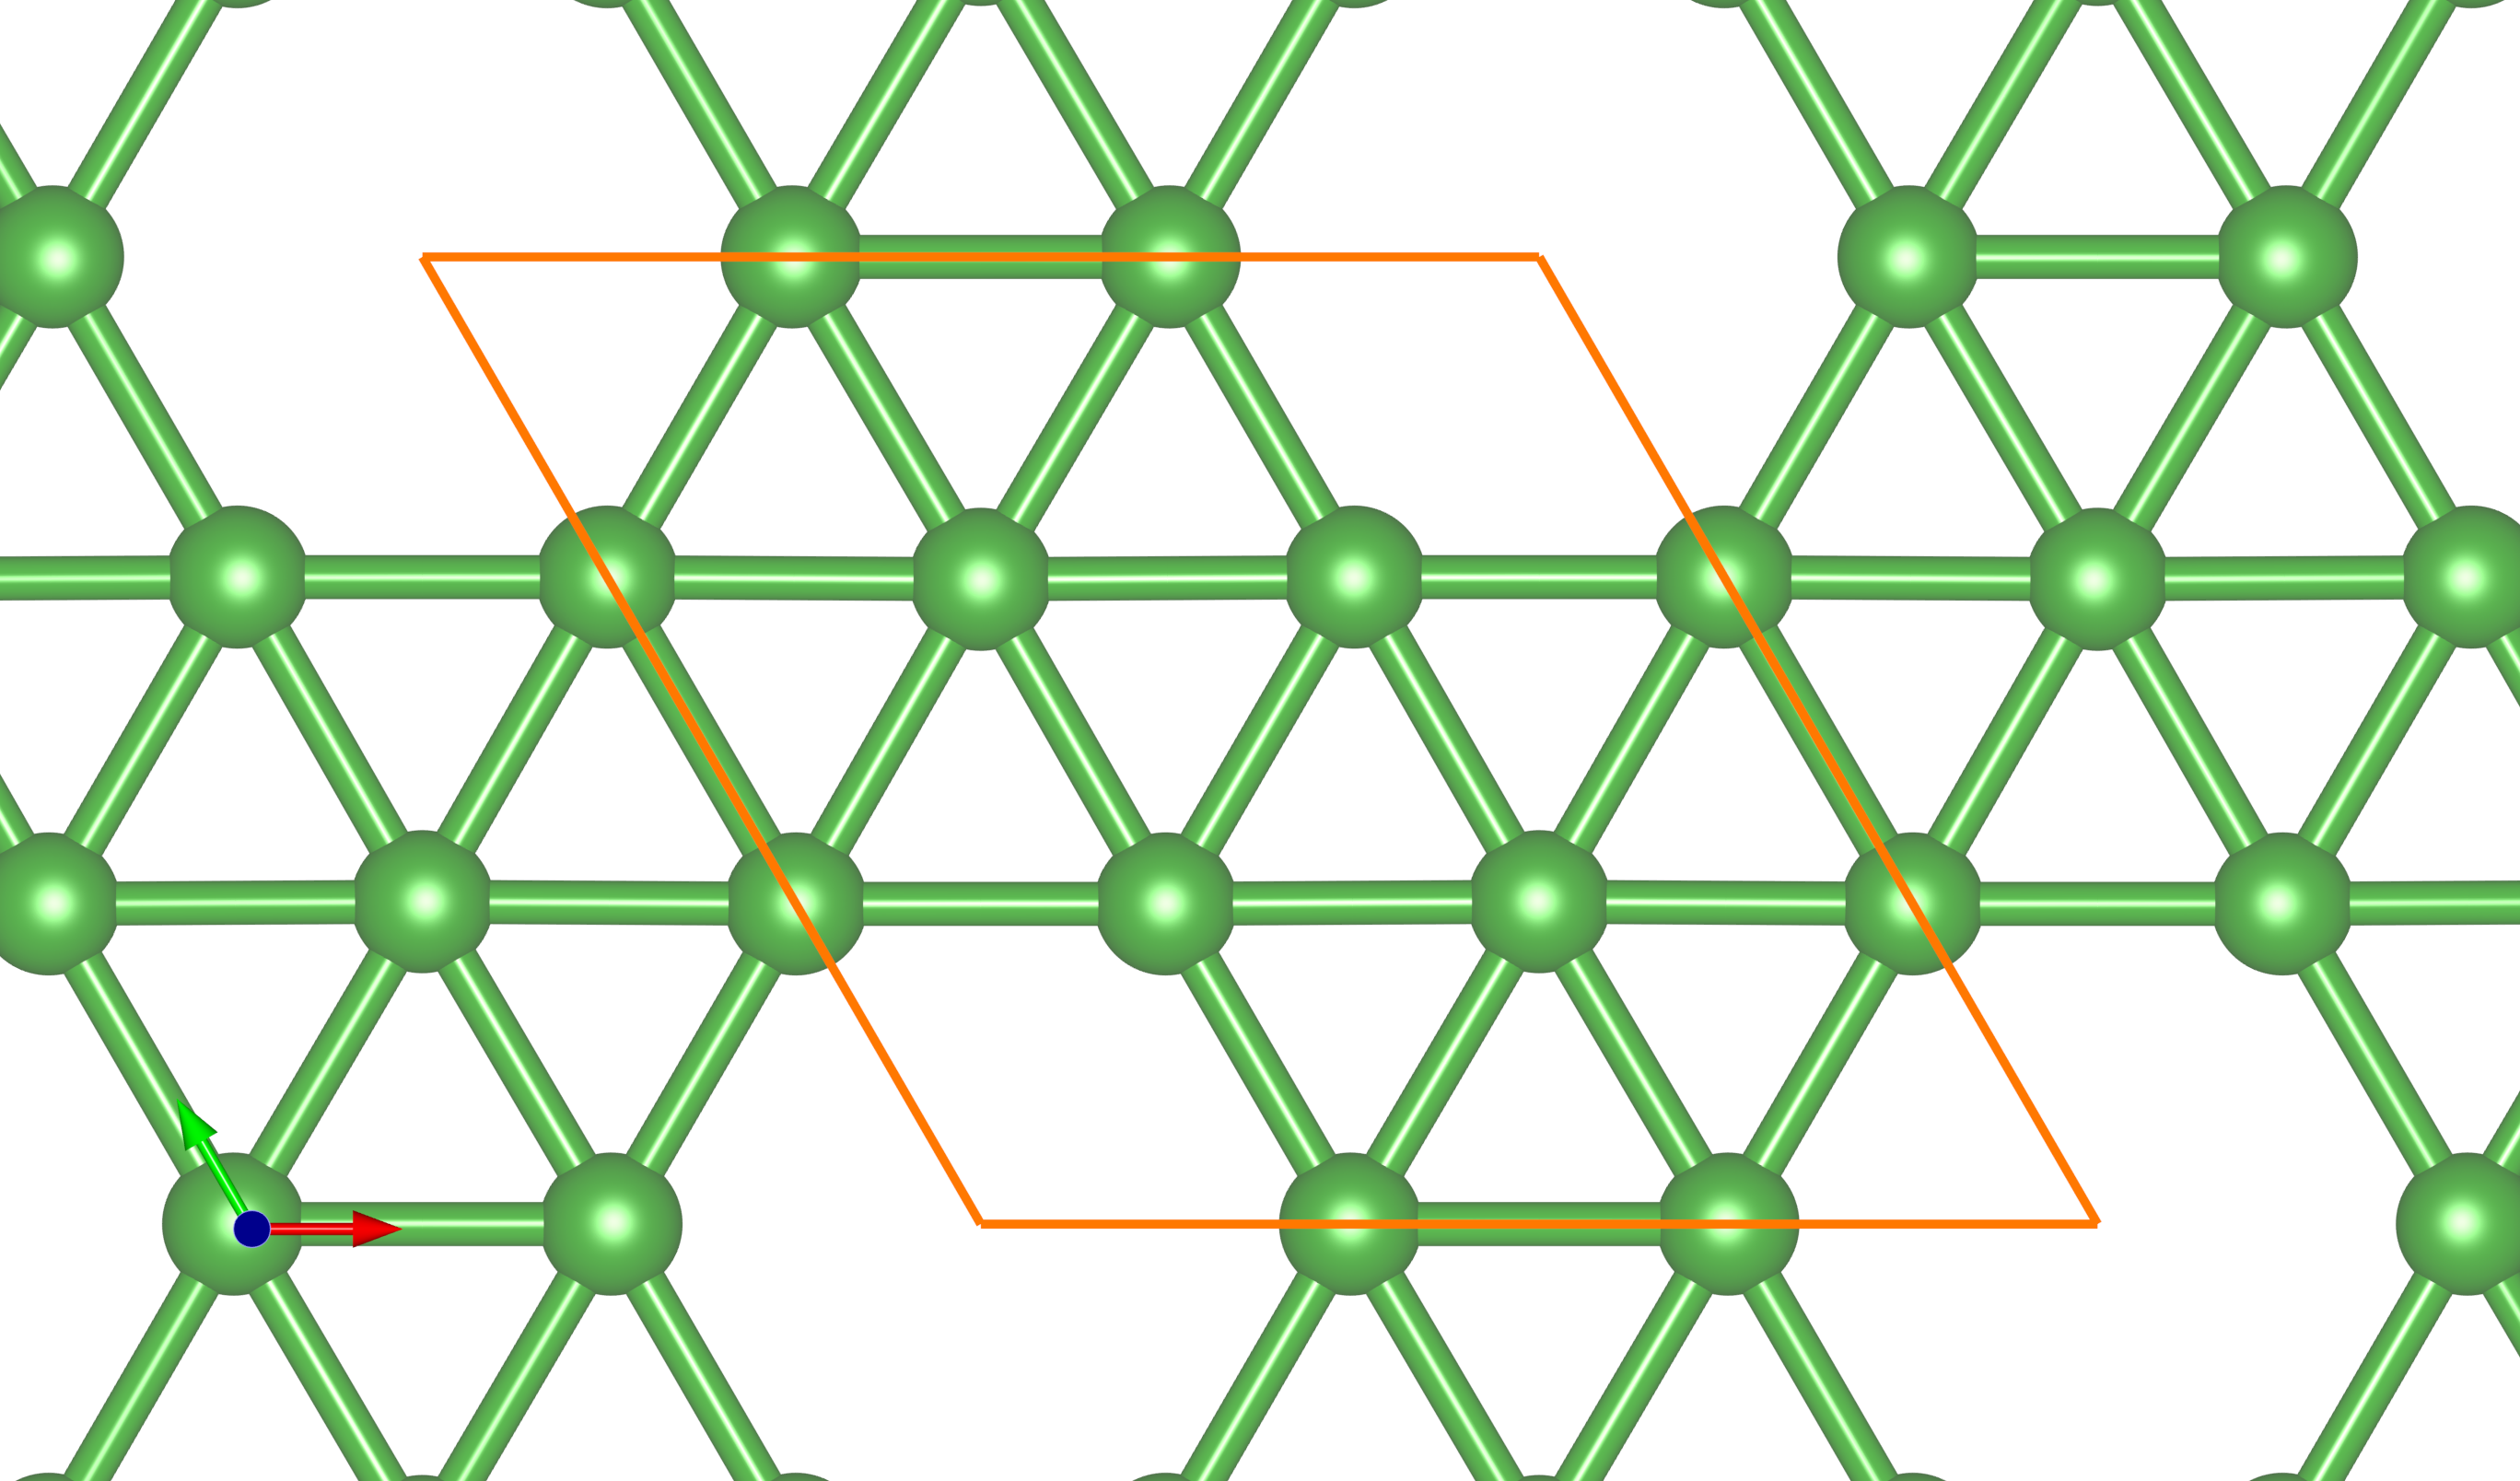
\includegraphics[width=0.5\textwidth]{Supercells/B_Borophene.png}
        \caption{Borophene supercell}
    \end{figure}\end{column}
    \begin{column}{0.5\textwidth}
        \par \textbf{Monolayer: Borophene}
        \par\quad LUMO band: -2.286900;
        \par\quad HOMO band: -1.730100;
        \par\quad Band gap: -0.556800.
    \end{column}
\end{columns}
\begin{columns}
    \begin{column}{0.45\textwidth}\begin{figure}
        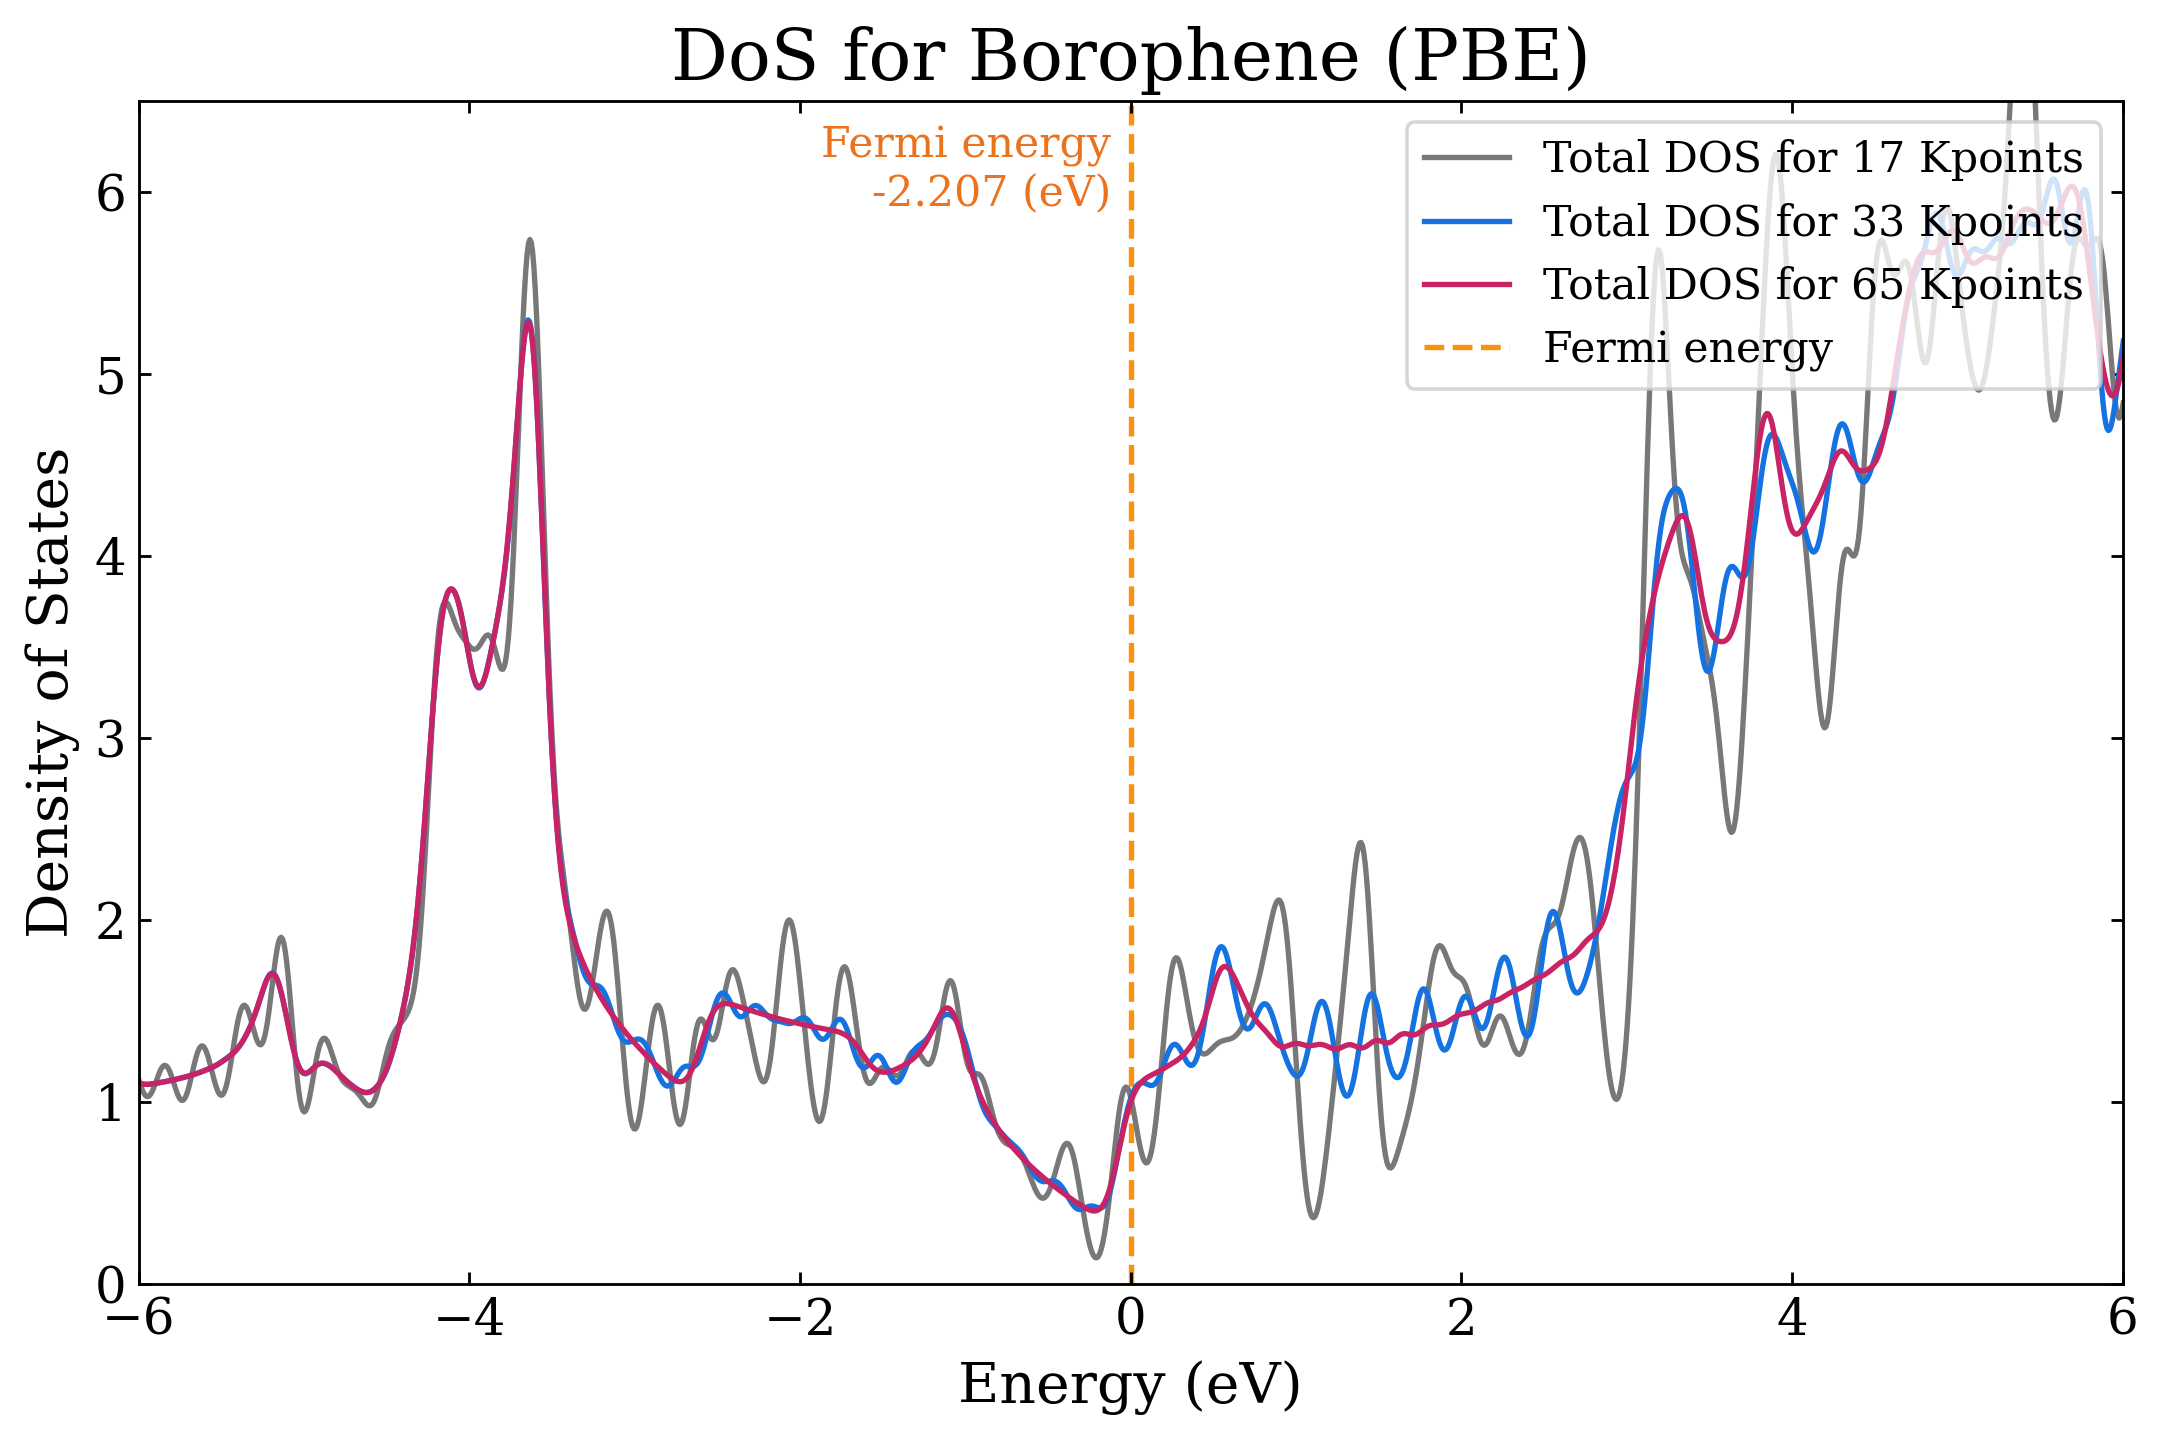
\includegraphics[width=1\textwidth]{PDoS/Borophene_dos.png}
        \caption{Borophene DoS}
    \end{figure}\end{column}
    \begin{column}{0.55\textwidth}\begin{figure}
        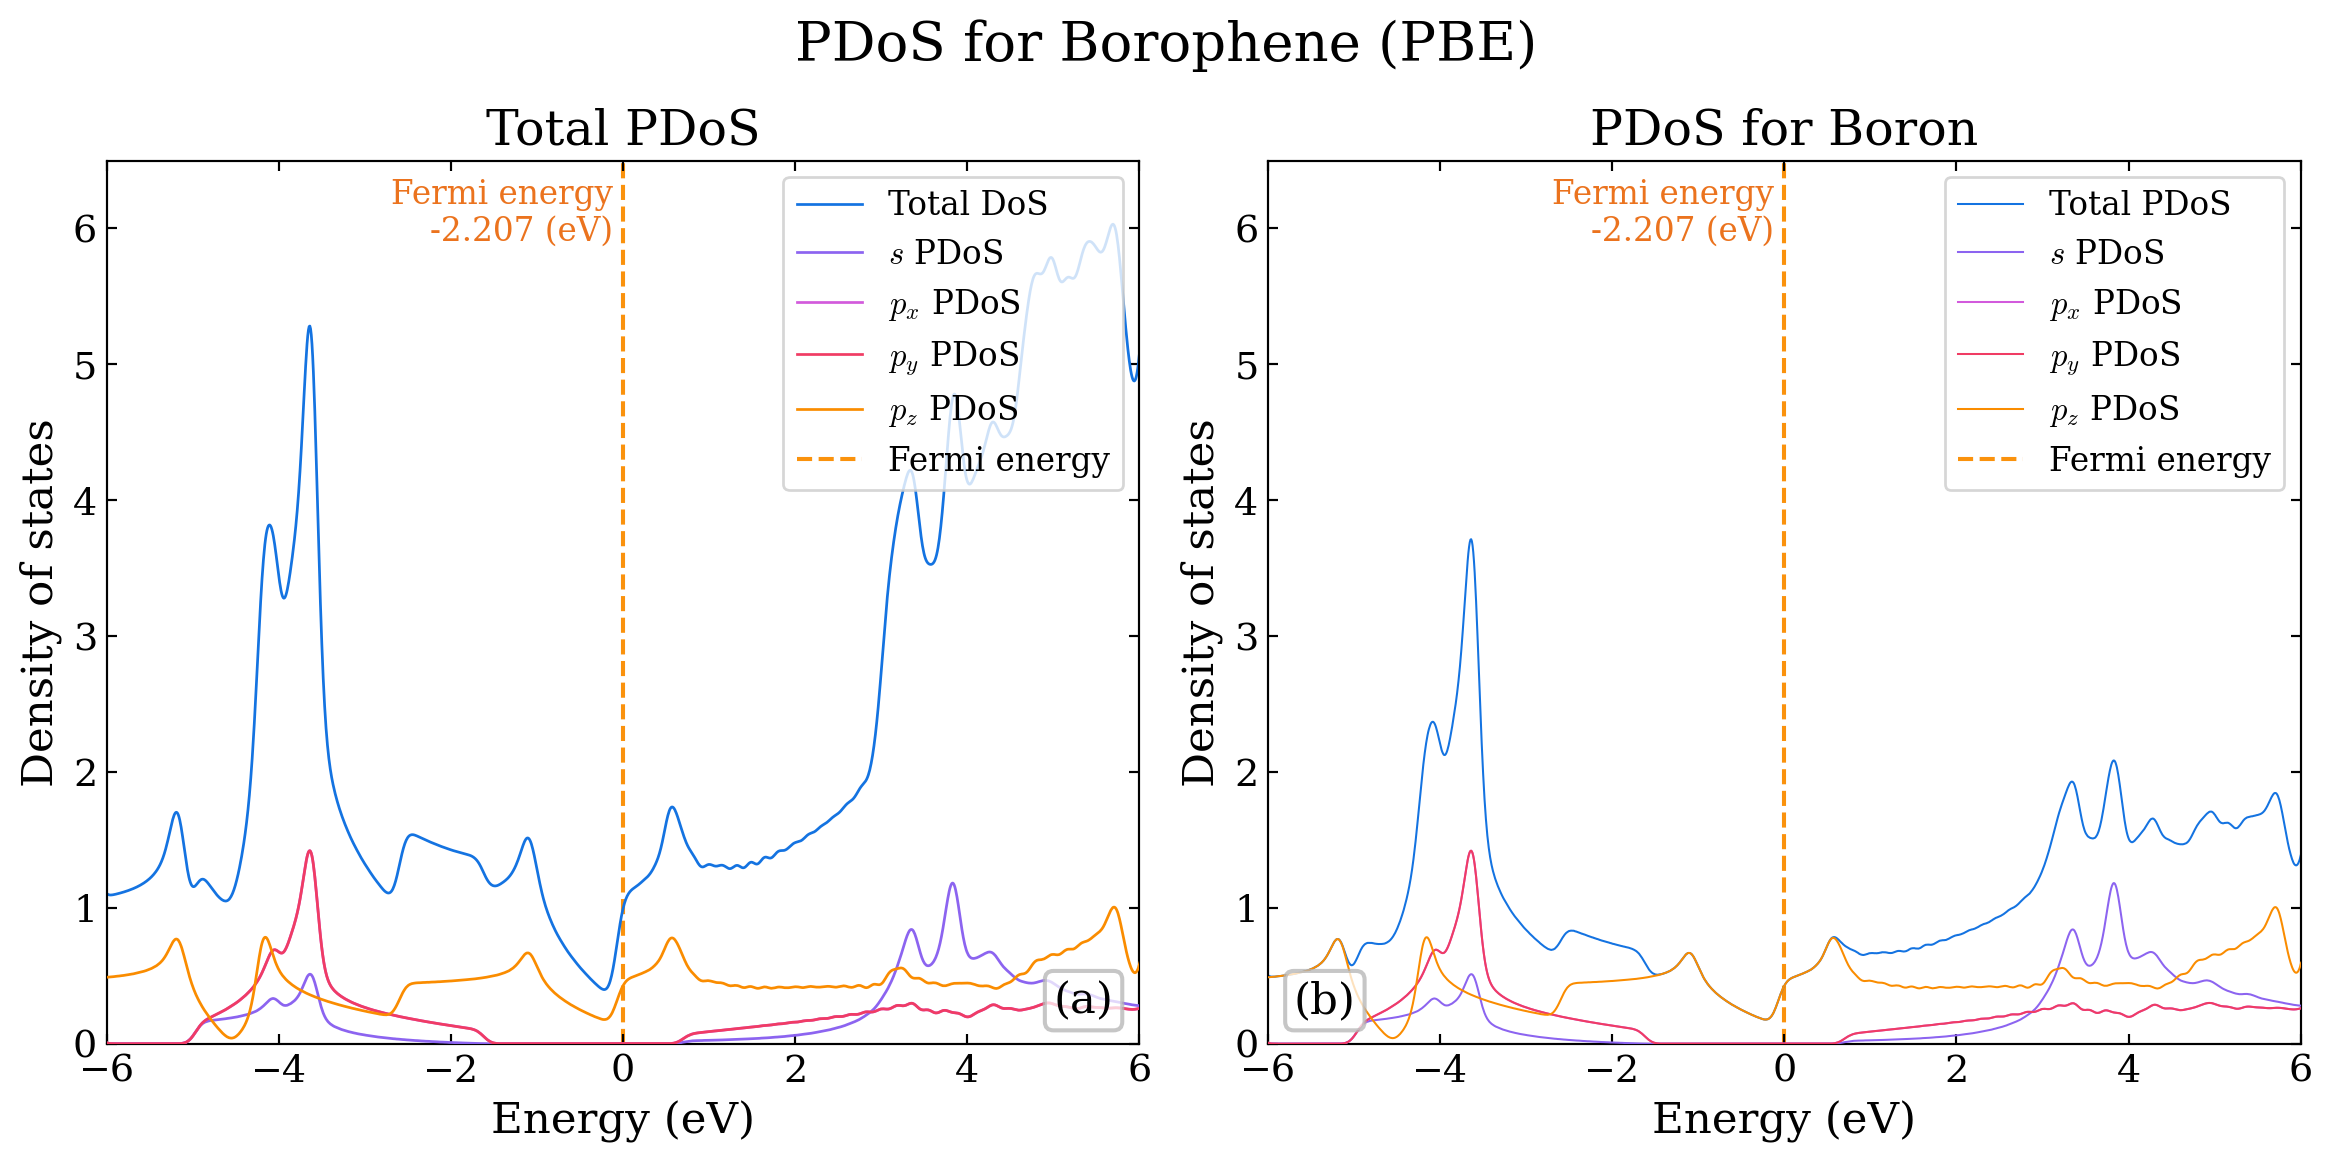
\includegraphics[width=0.8\textwidth]{PDoS/Borophene_pdos.png}
        \caption{Borophene PDoS}
    \end{figure}\end{column}
\end{columns}
\end{frame}

\subsection{B\texorpdfstring{$_\text{4}$}{4}C\texorpdfstring{$_\text{3}$}{3} (PBE)}
\begin{frame}{\insertsection: \insertsubsection}
\begin{columns}
    \begin{column}{0.5\textwidth}\begin{figure}
        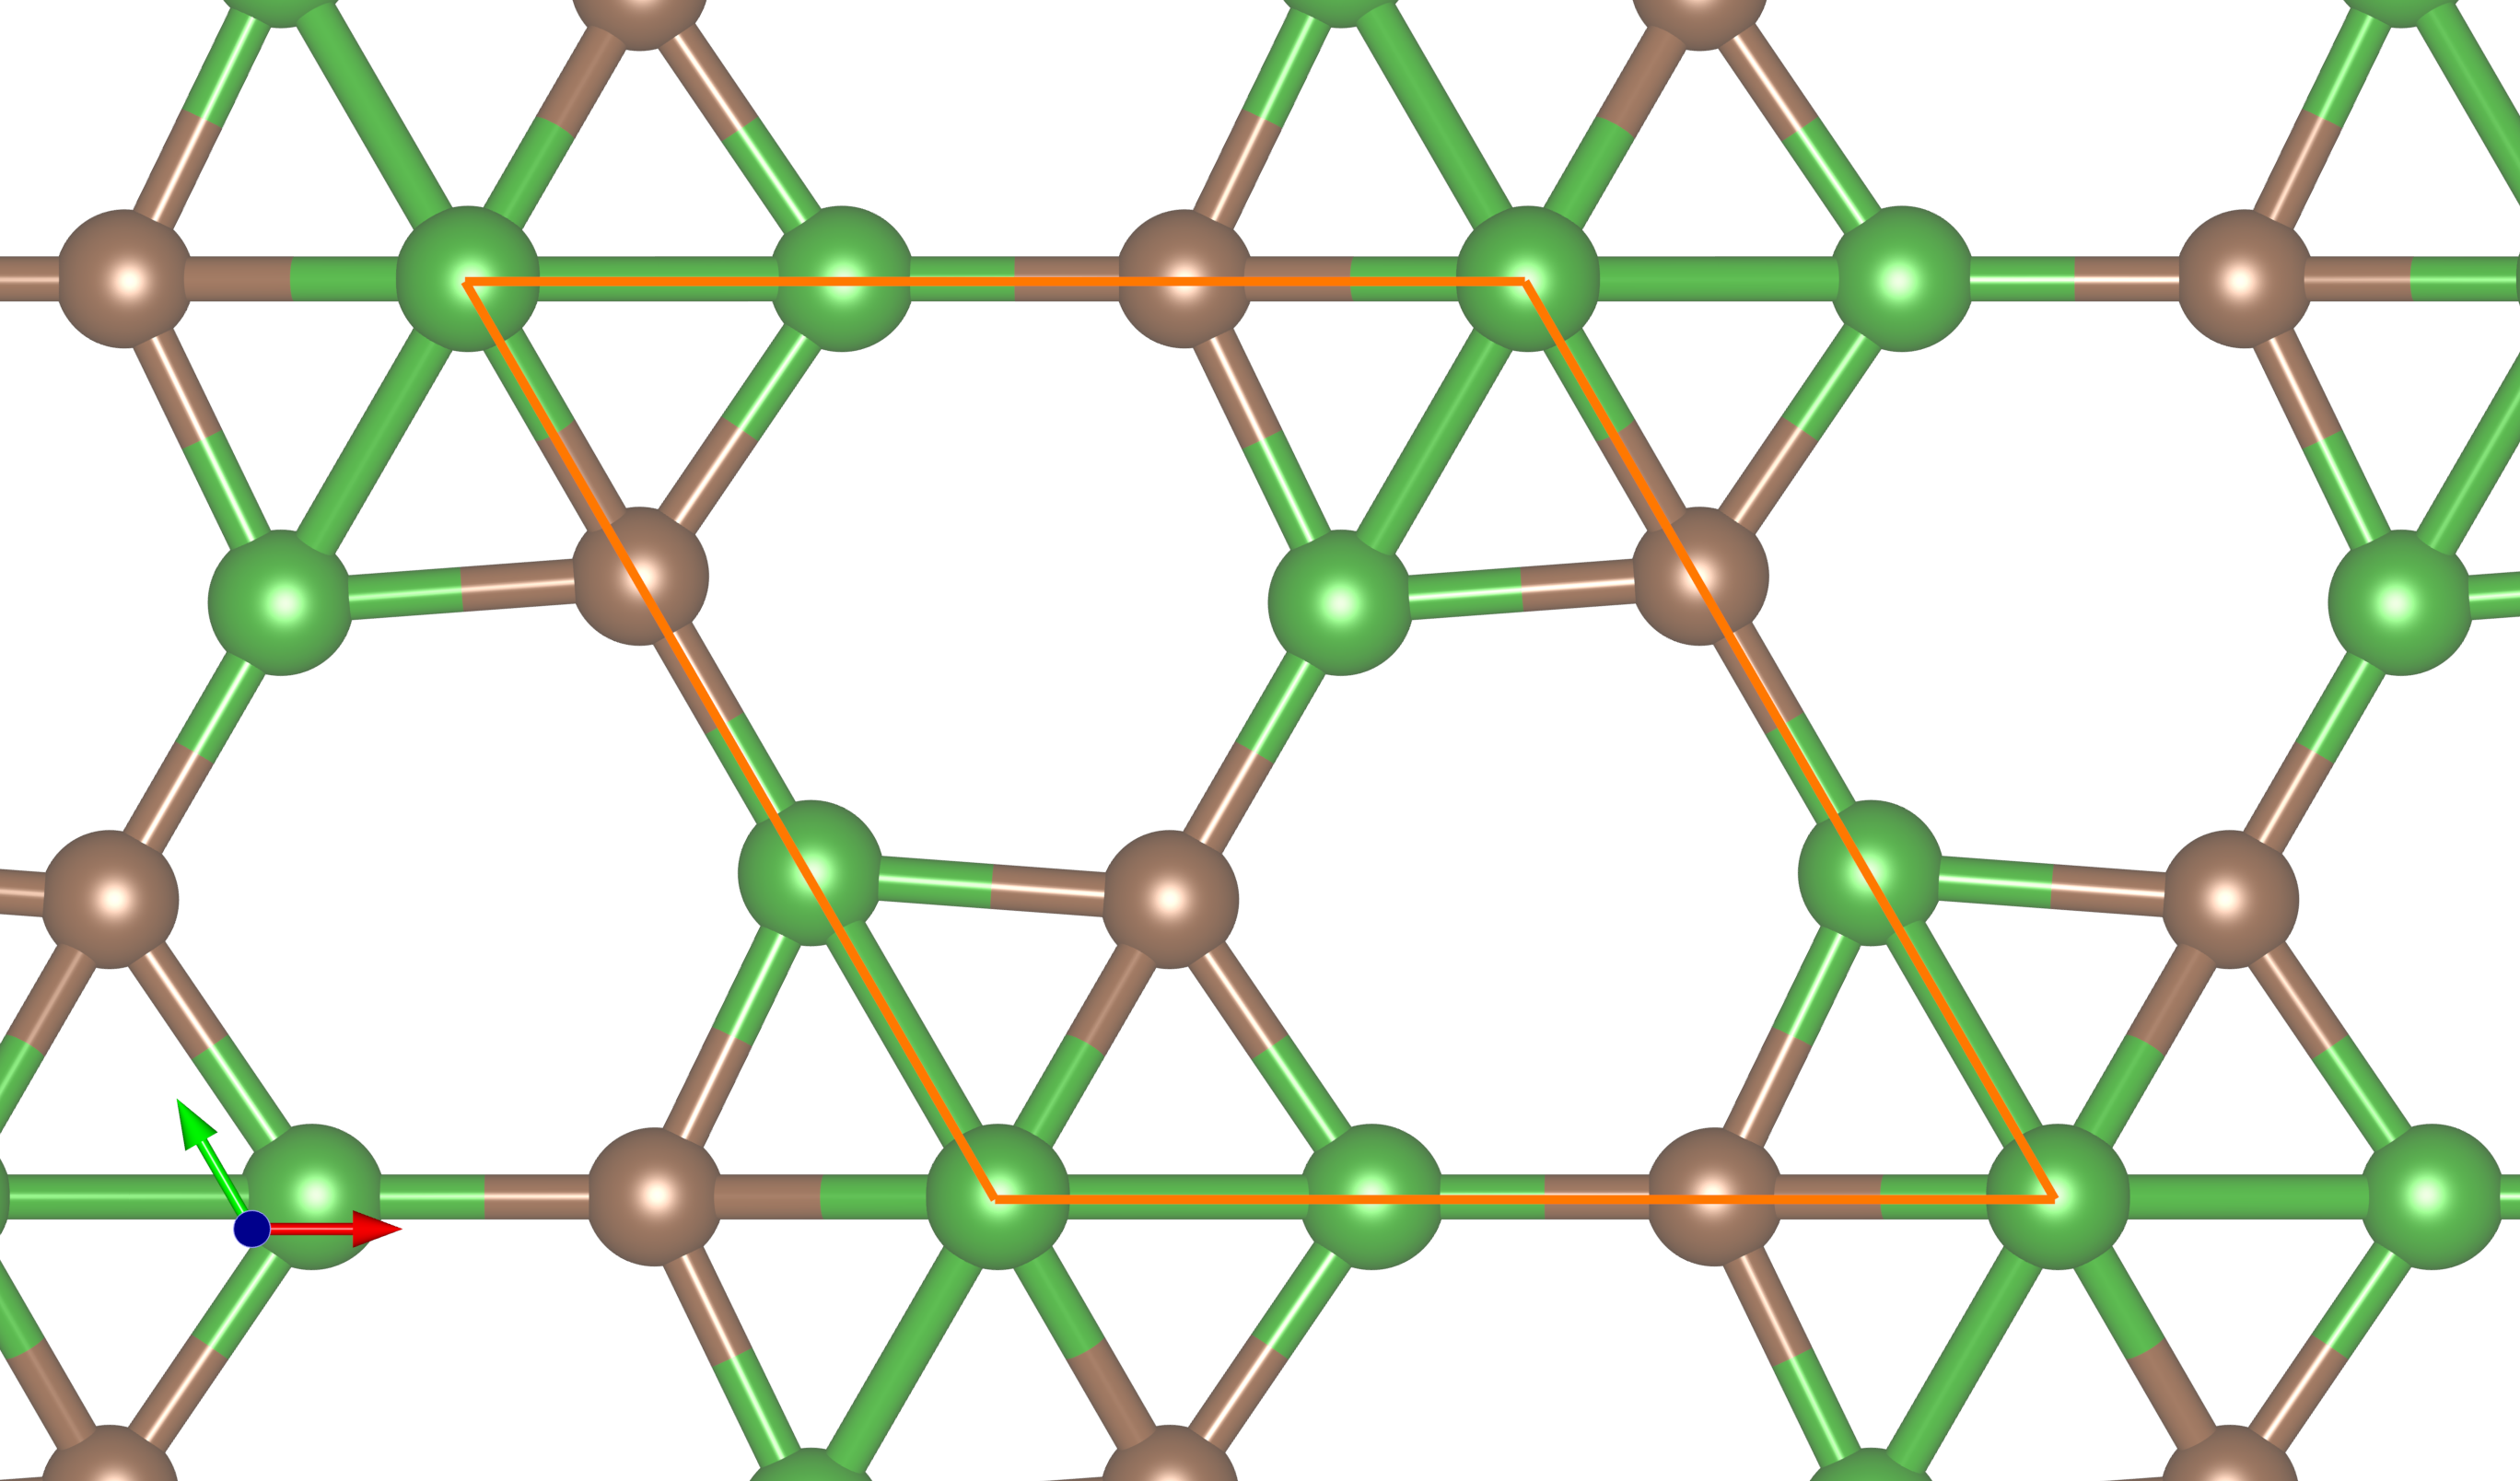
\includegraphics[width=0.5\textwidth]{Supercells/C_B4C3.png}
        \caption{B$_\text{4}$C$_\text{3}$ supercell}
    \end{figure}\end{column}
    \begin{column}{0.5\textwidth}
        \par \textbf{Monolayer: B$_\text{4}$C$_\text{3}$}
        \par\quad LUMO band: -1.209400;
        \par\quad HOMO band: -2.855900;
        \par\quad Band gap: 1.646500.
    \end{column}
\end{columns}
\begin{columns}
    \begin{column}{0.45\textwidth}\begin{figure}
        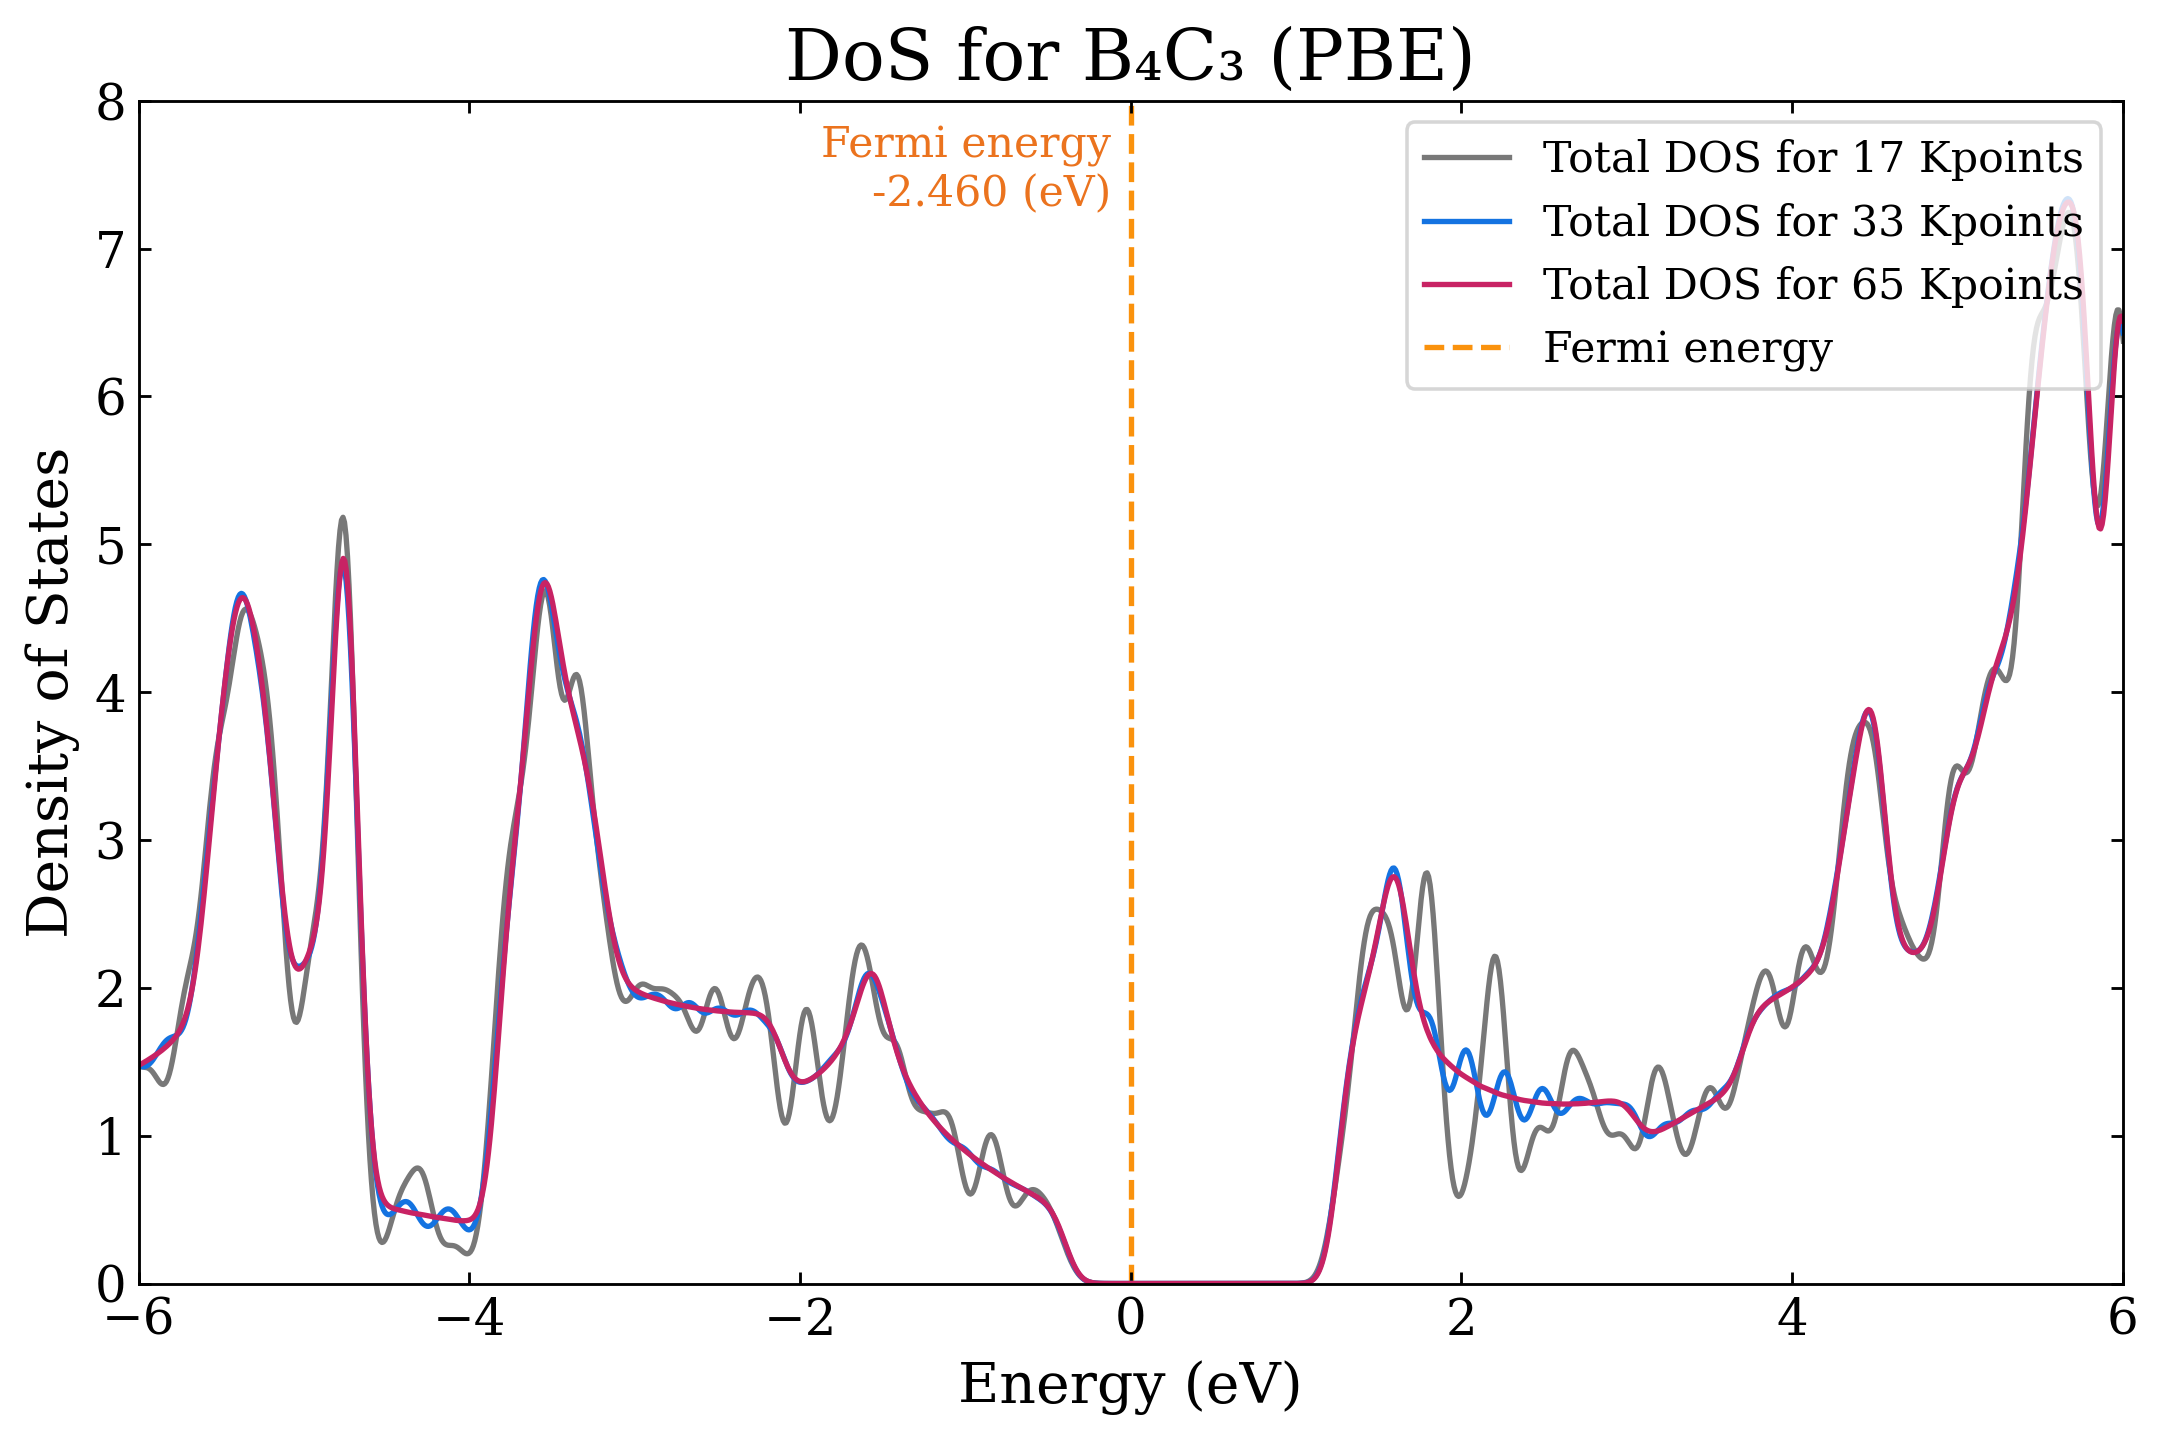
\includegraphics[width=1\textwidth]{PDoS/B4C3_dos}
        \caption{B$_\text{4}$C$_\text{3}$ DoS}
    \end{figure}\end{column}
    \begin{column}{0.55\textwidth}\begin{figure}
        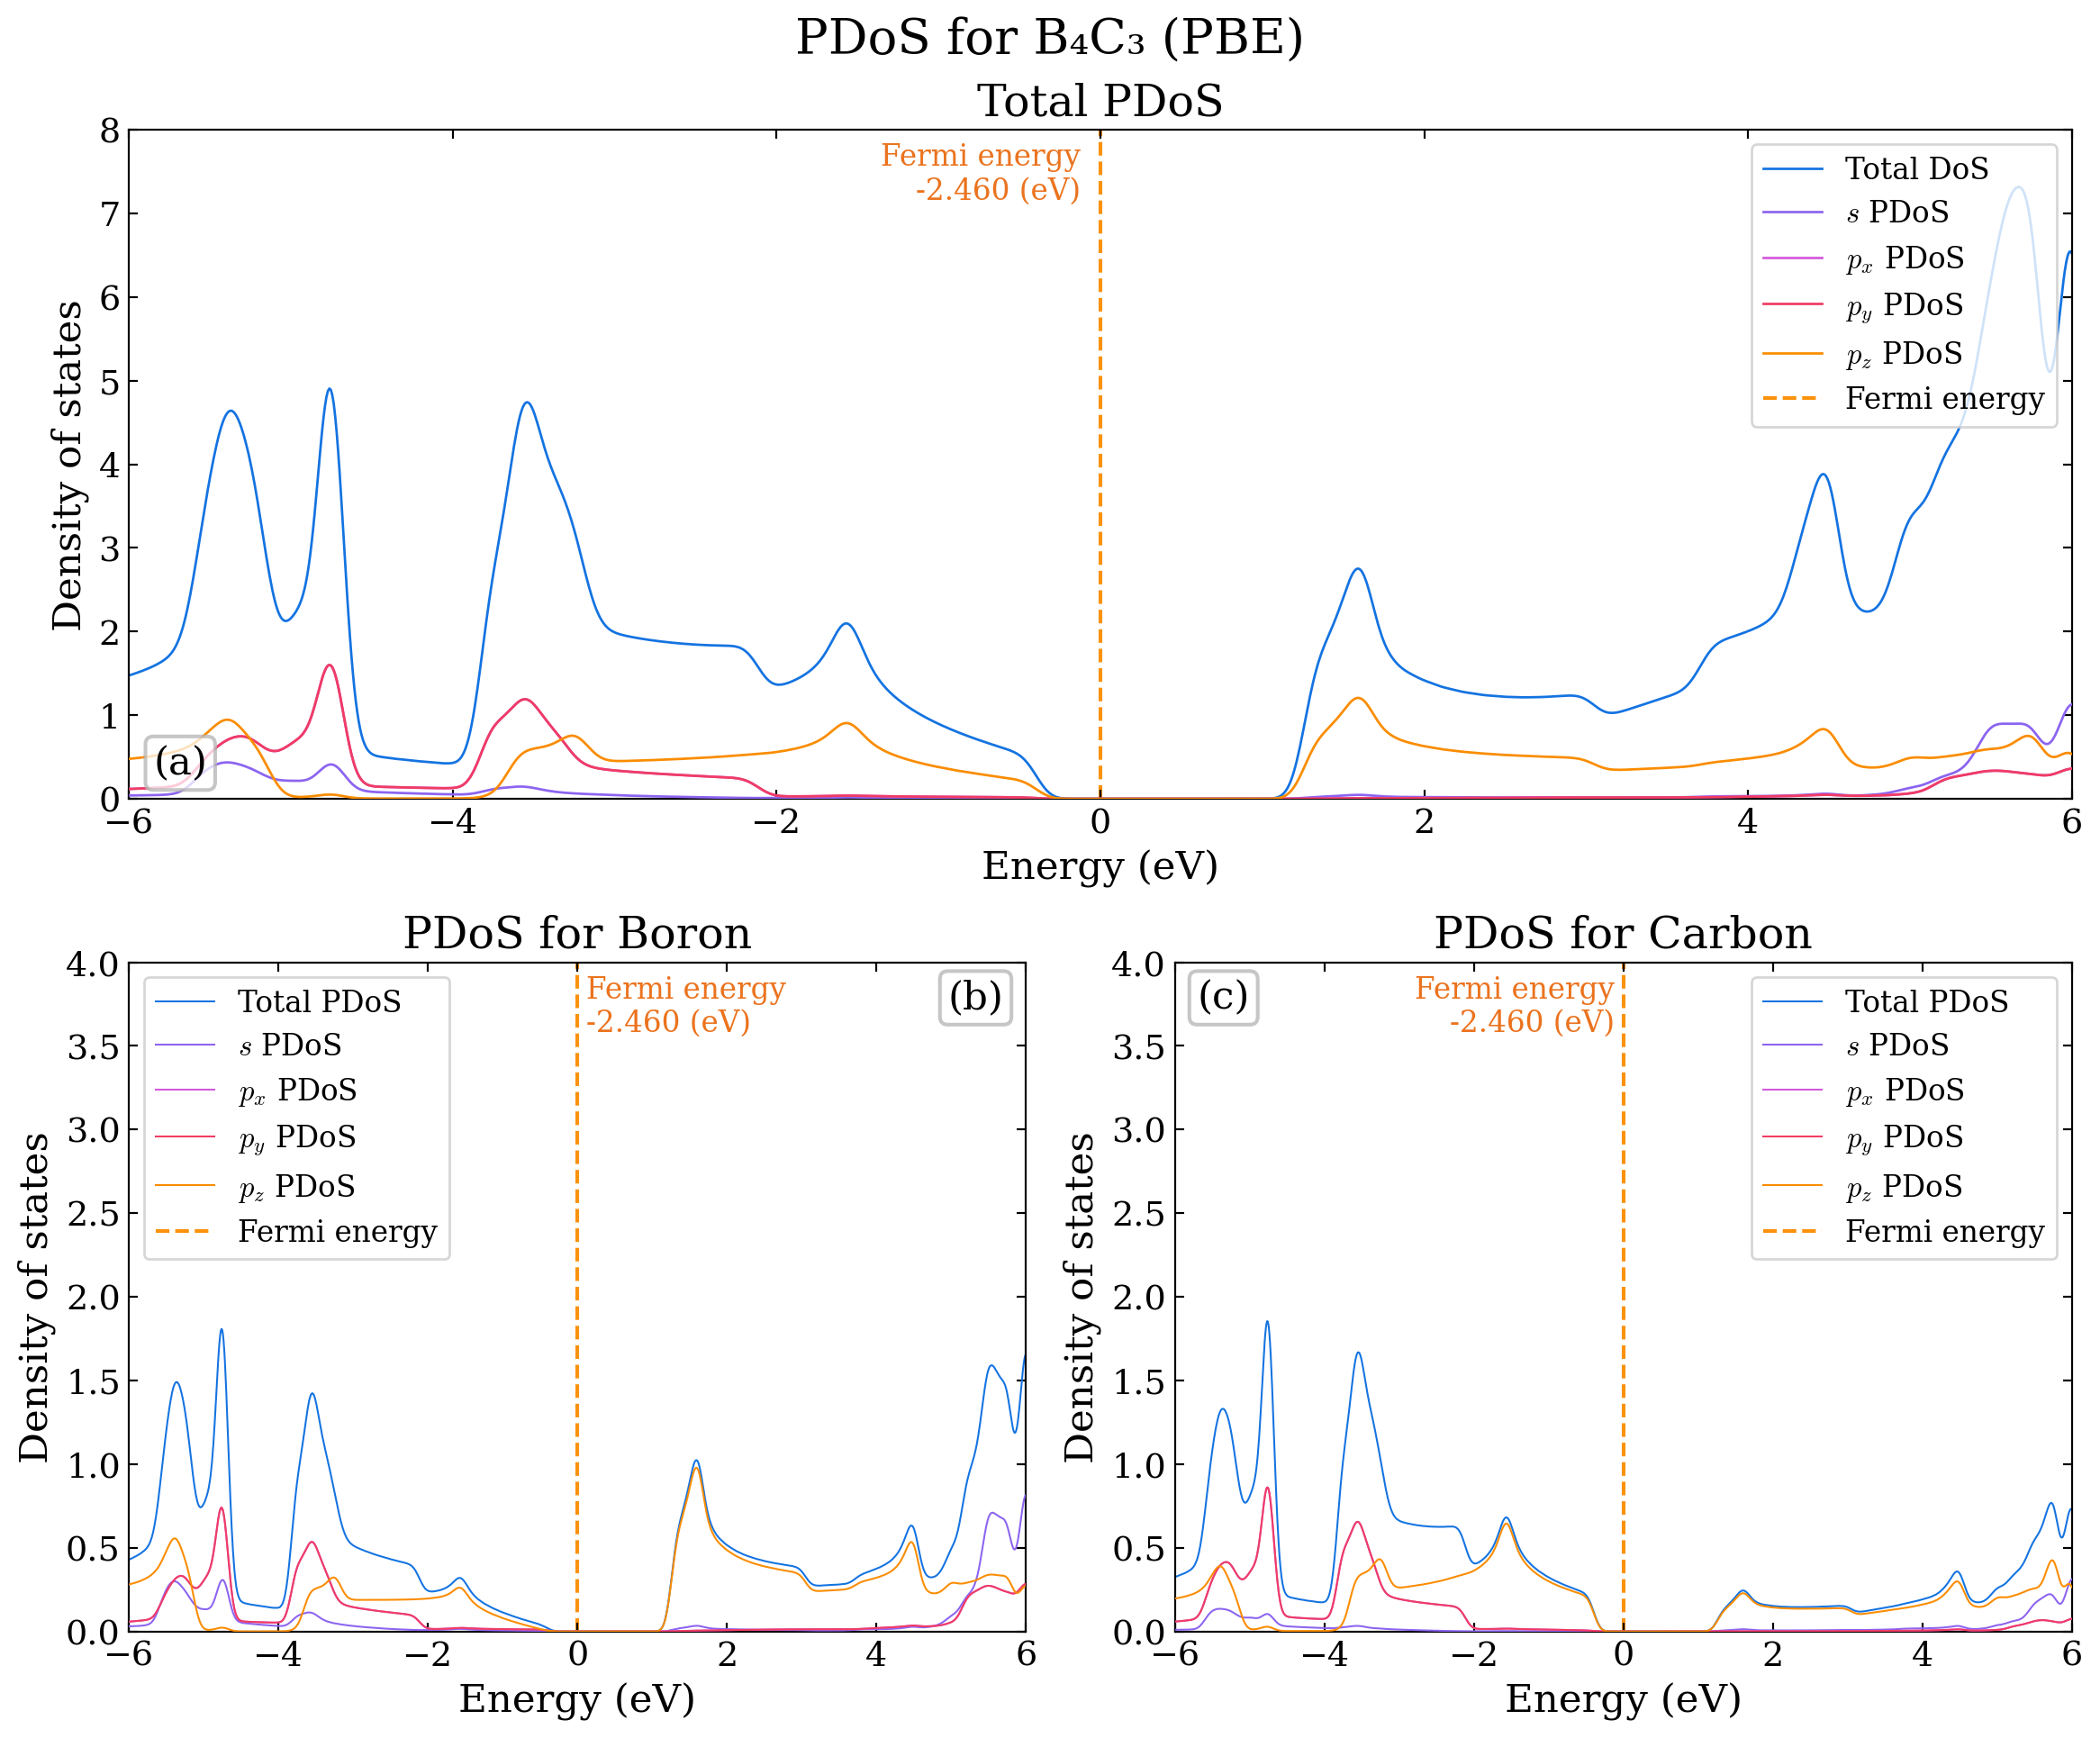
\includegraphics[width=0.8\textwidth]{PDoS/B4C3_pdos.png}
        \caption{B$_\text{4}$C$_\text{3}$ PDoS}
    \end{figure}\end{column}
\end{columns}
\end{frame}

\subsection{Graphene (PBE)}
\begin{frame}{\insertsection: \insertsubsection}
\begin{columns}
    \begin{column}{0.5\textwidth}\begin{figure}
        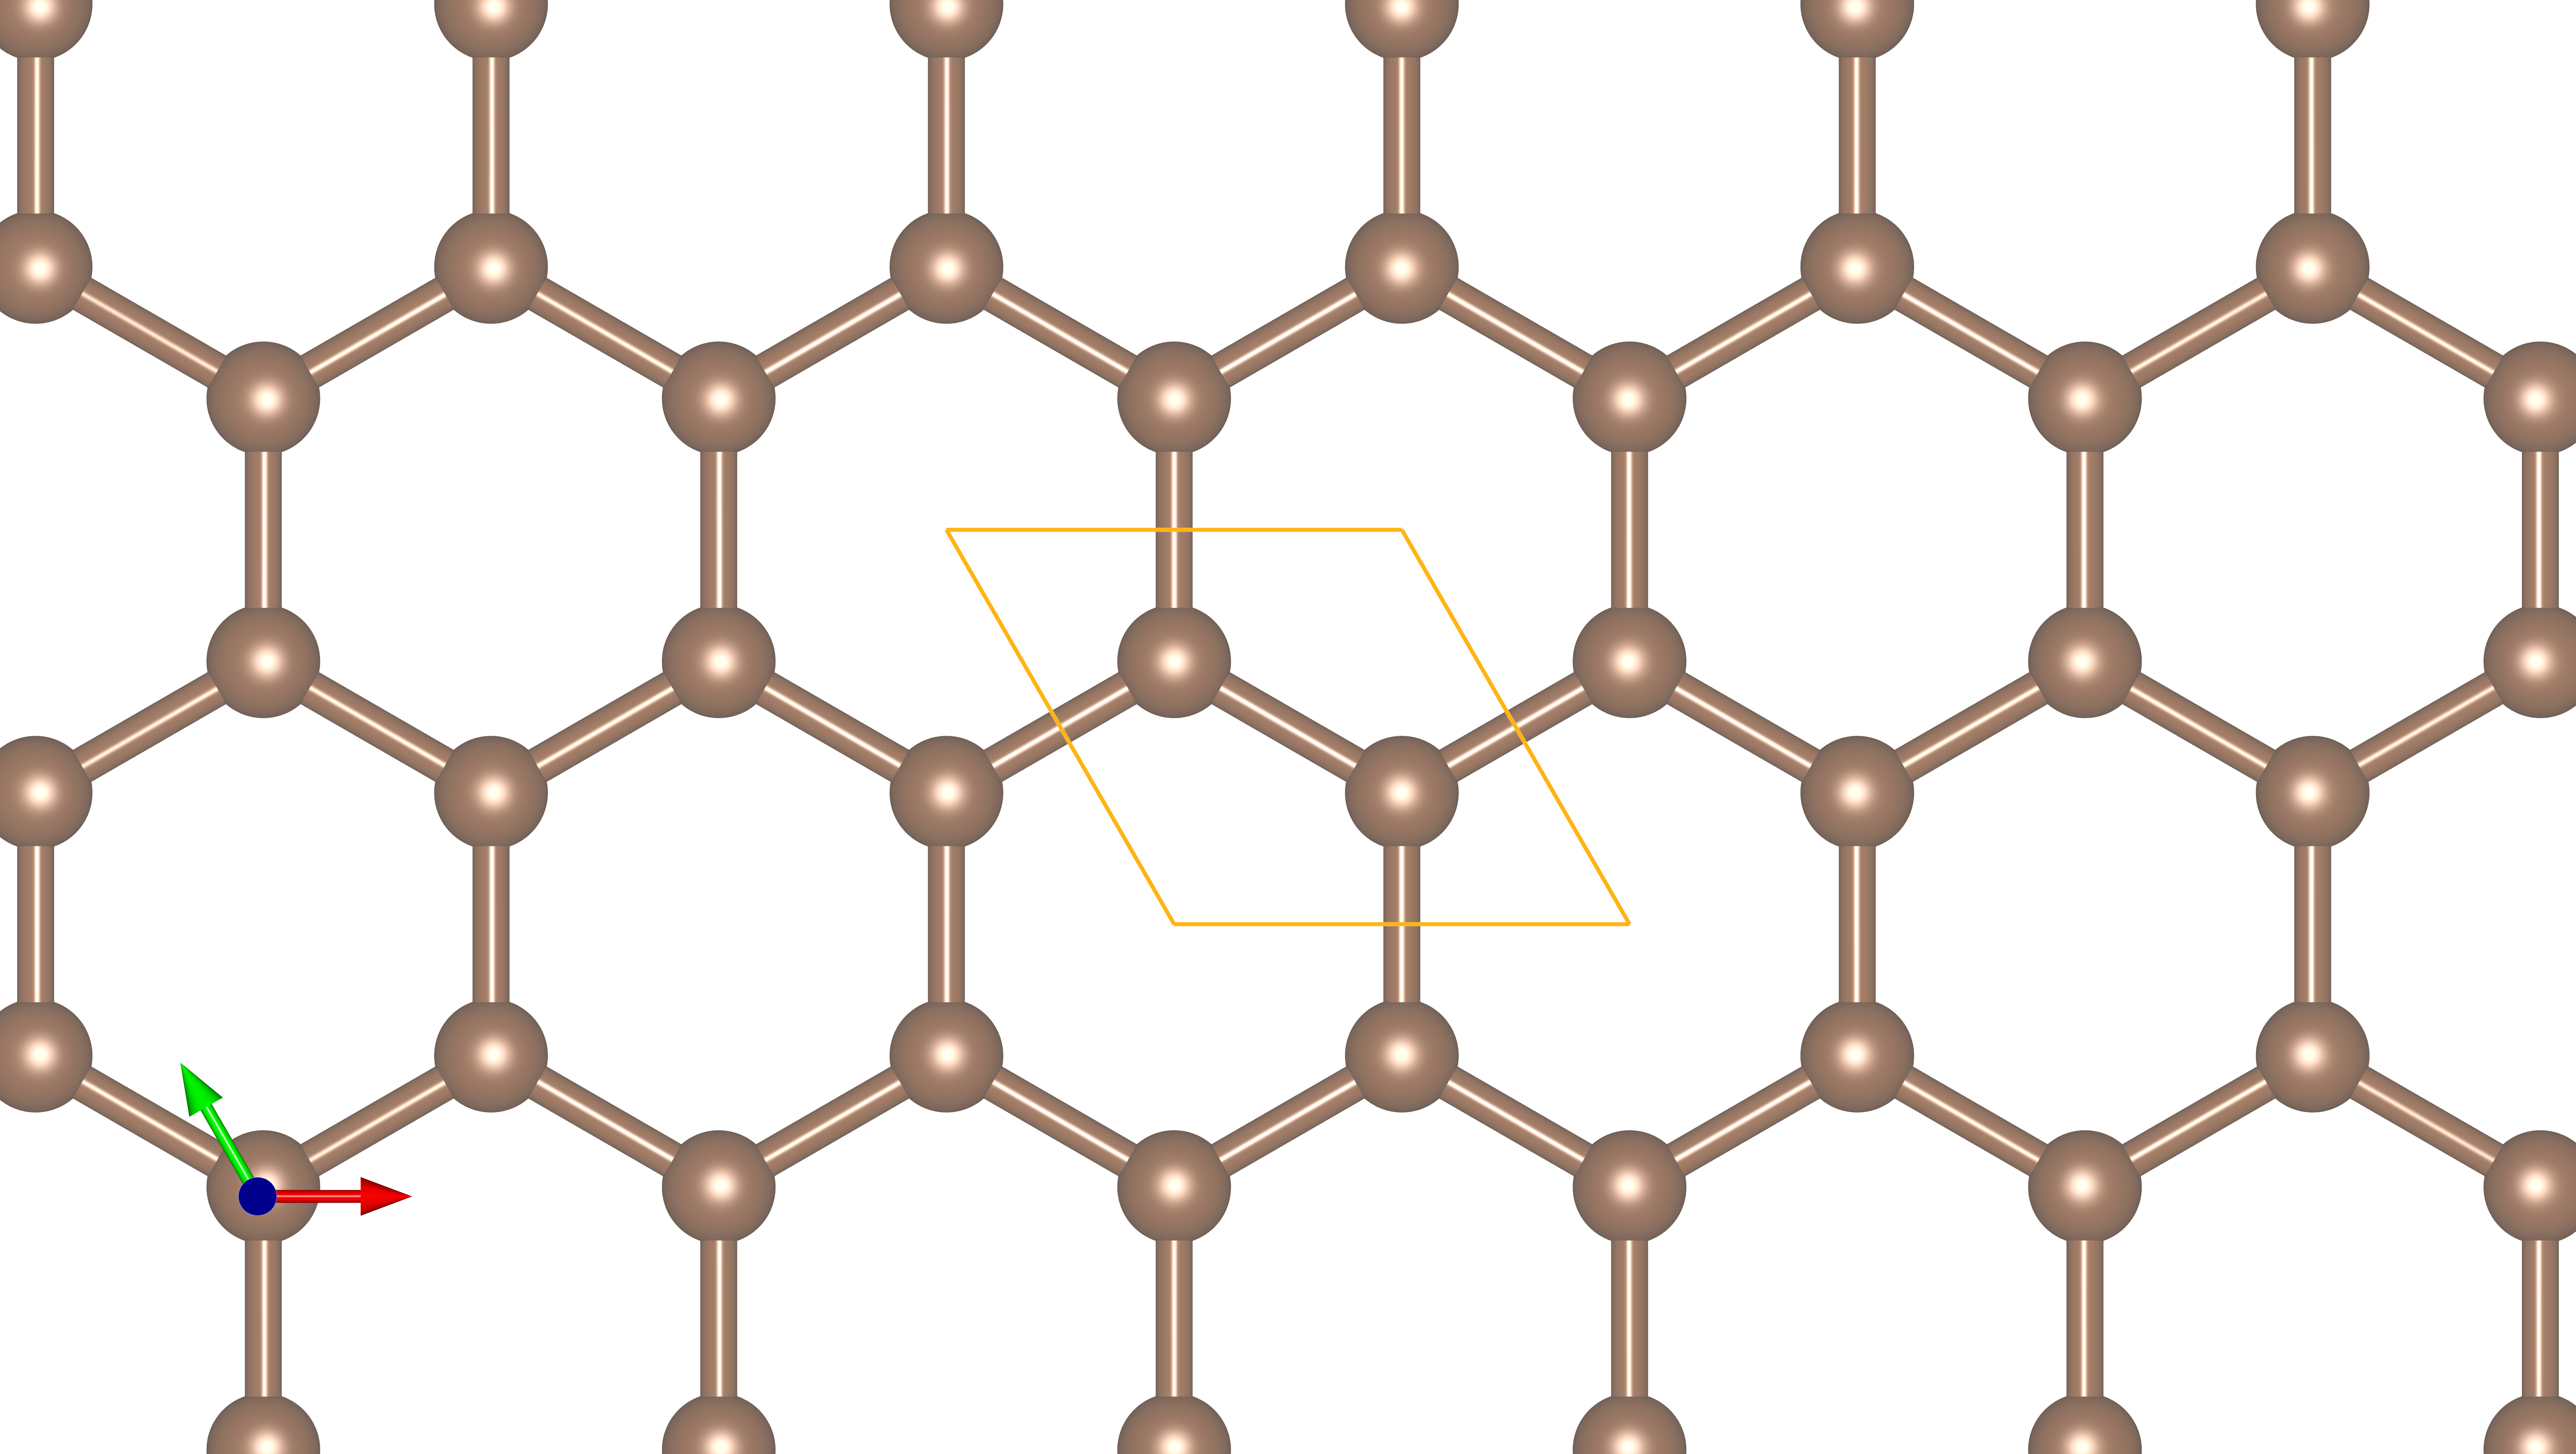
\includegraphics[width=0.5\textwidth]{Supercells/D_Graphene.png}
        \caption{Graphene supercell}
    \end{figure}\end{column}
    \begin{column}{0.5\textwidth}
        \par \textbf{Monolayer: Graphene}
        \par\quad LUMO band: -2.243900;
        \par\quad HOMO band: -2.262400;
        \par\quad Band gap: 0.018500.
    \end{column}
\end{columns}
\begin{columns}
    \begin{column}{0.45\textwidth}\begin{figure}
        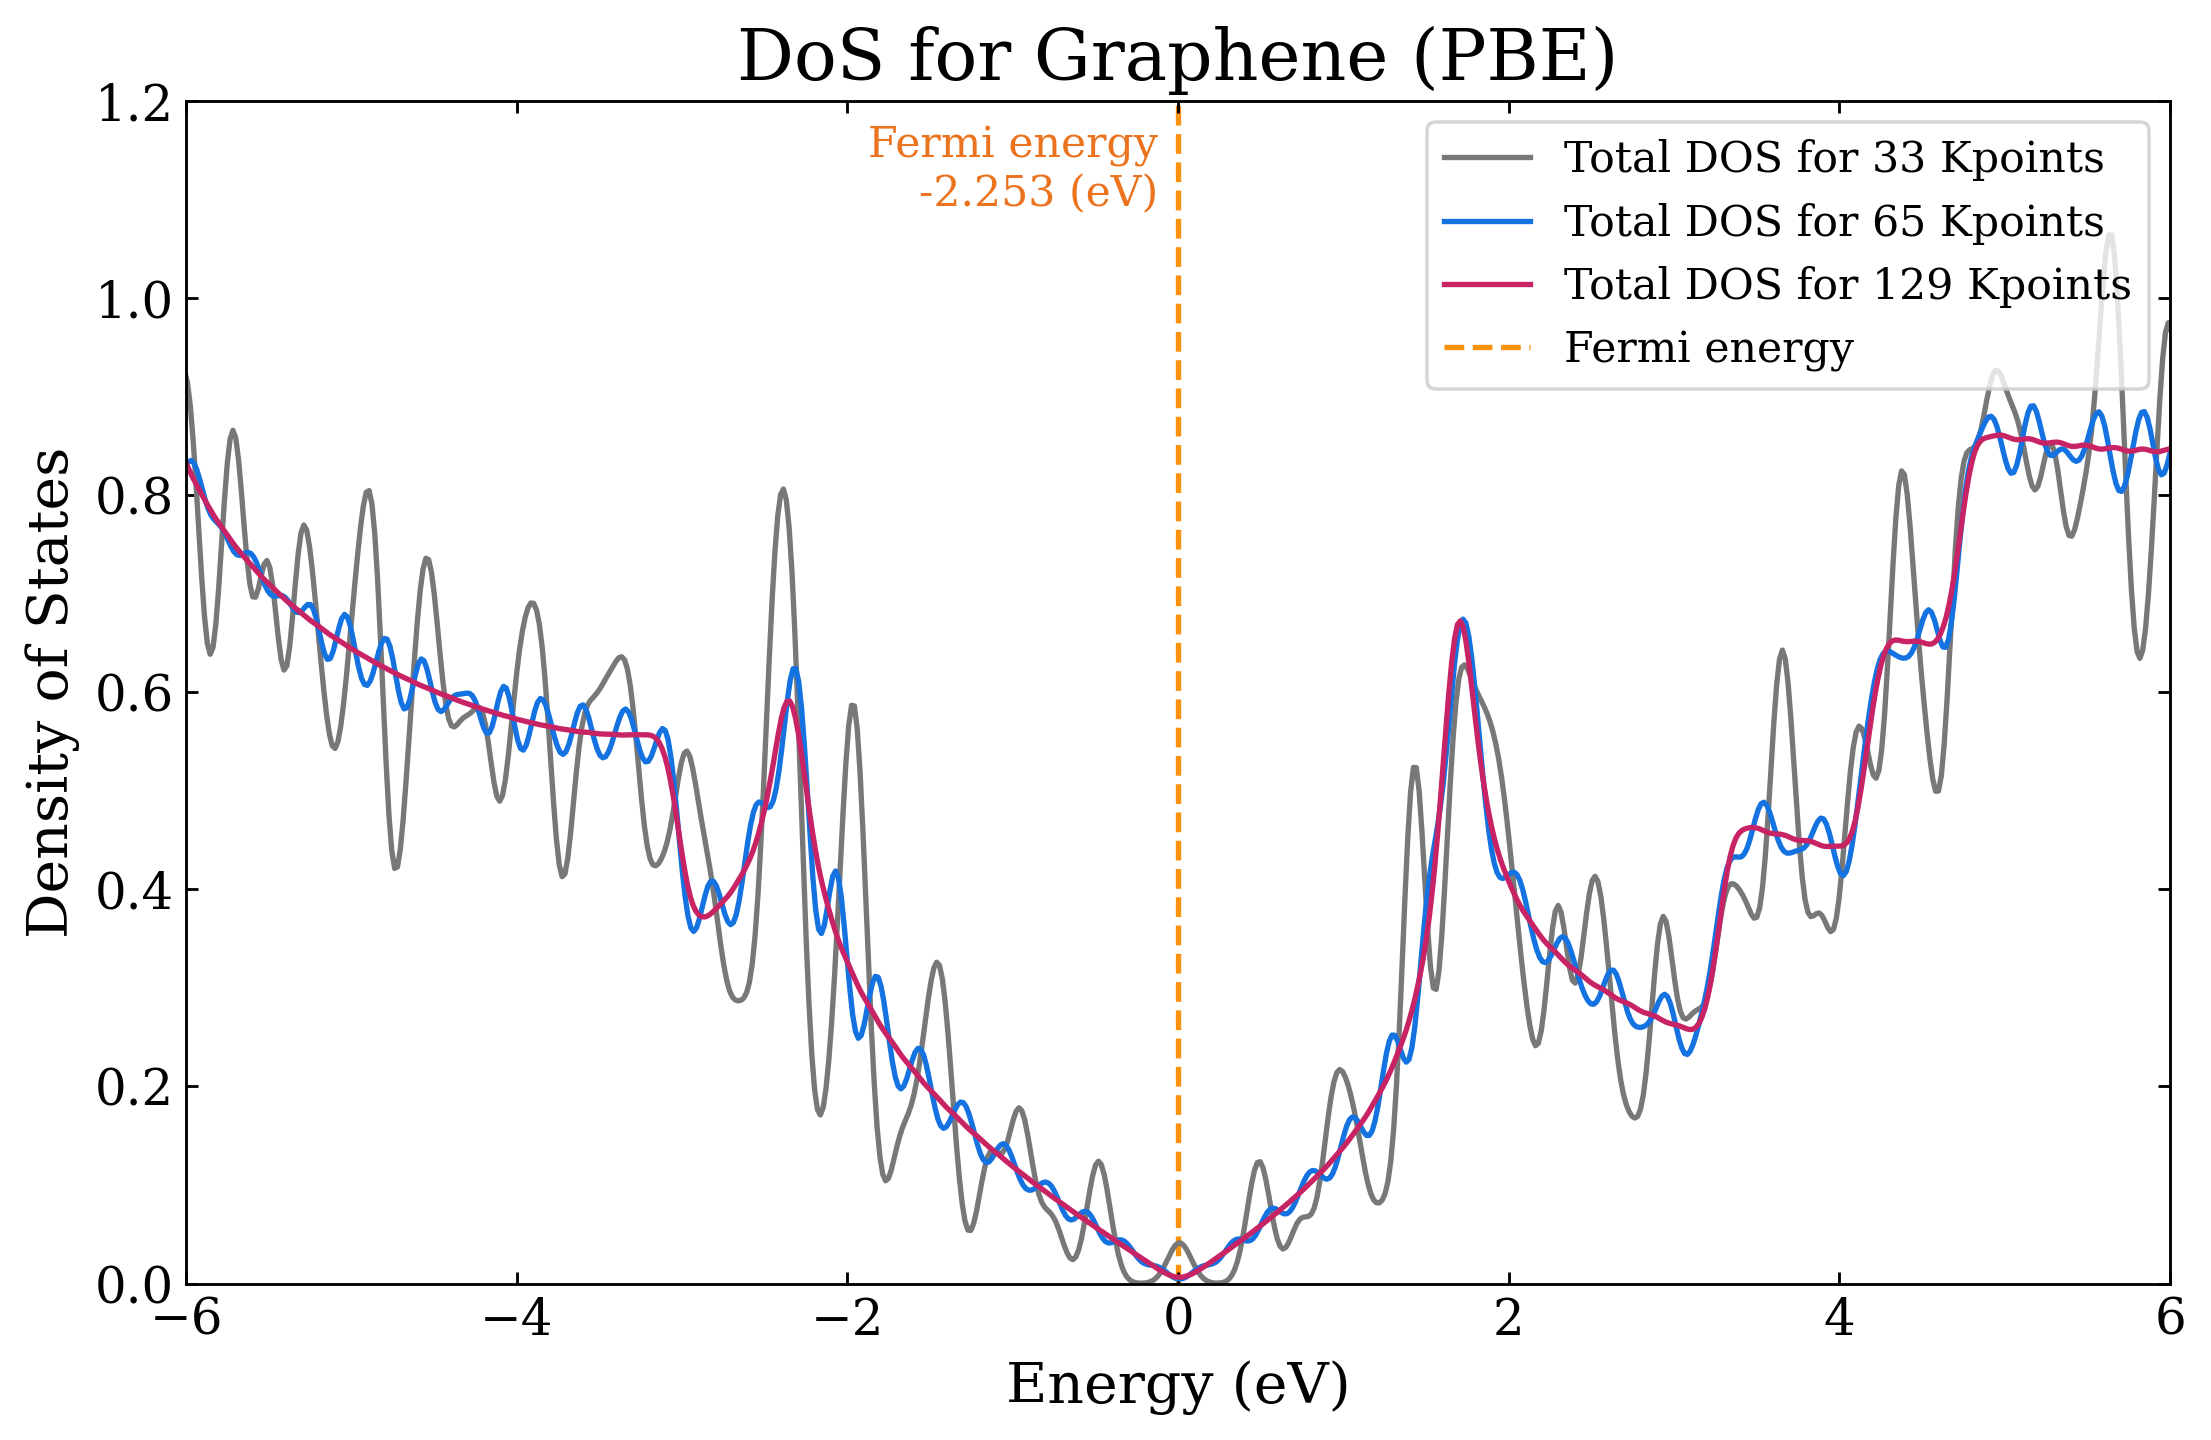
\includegraphics[width=1\textwidth]{PDoS/Graphene_dos}
        \caption{Graphene DoS}
    \end{figure}\end{column}
    \begin{column}{0.55\textwidth}\begin{figure}
        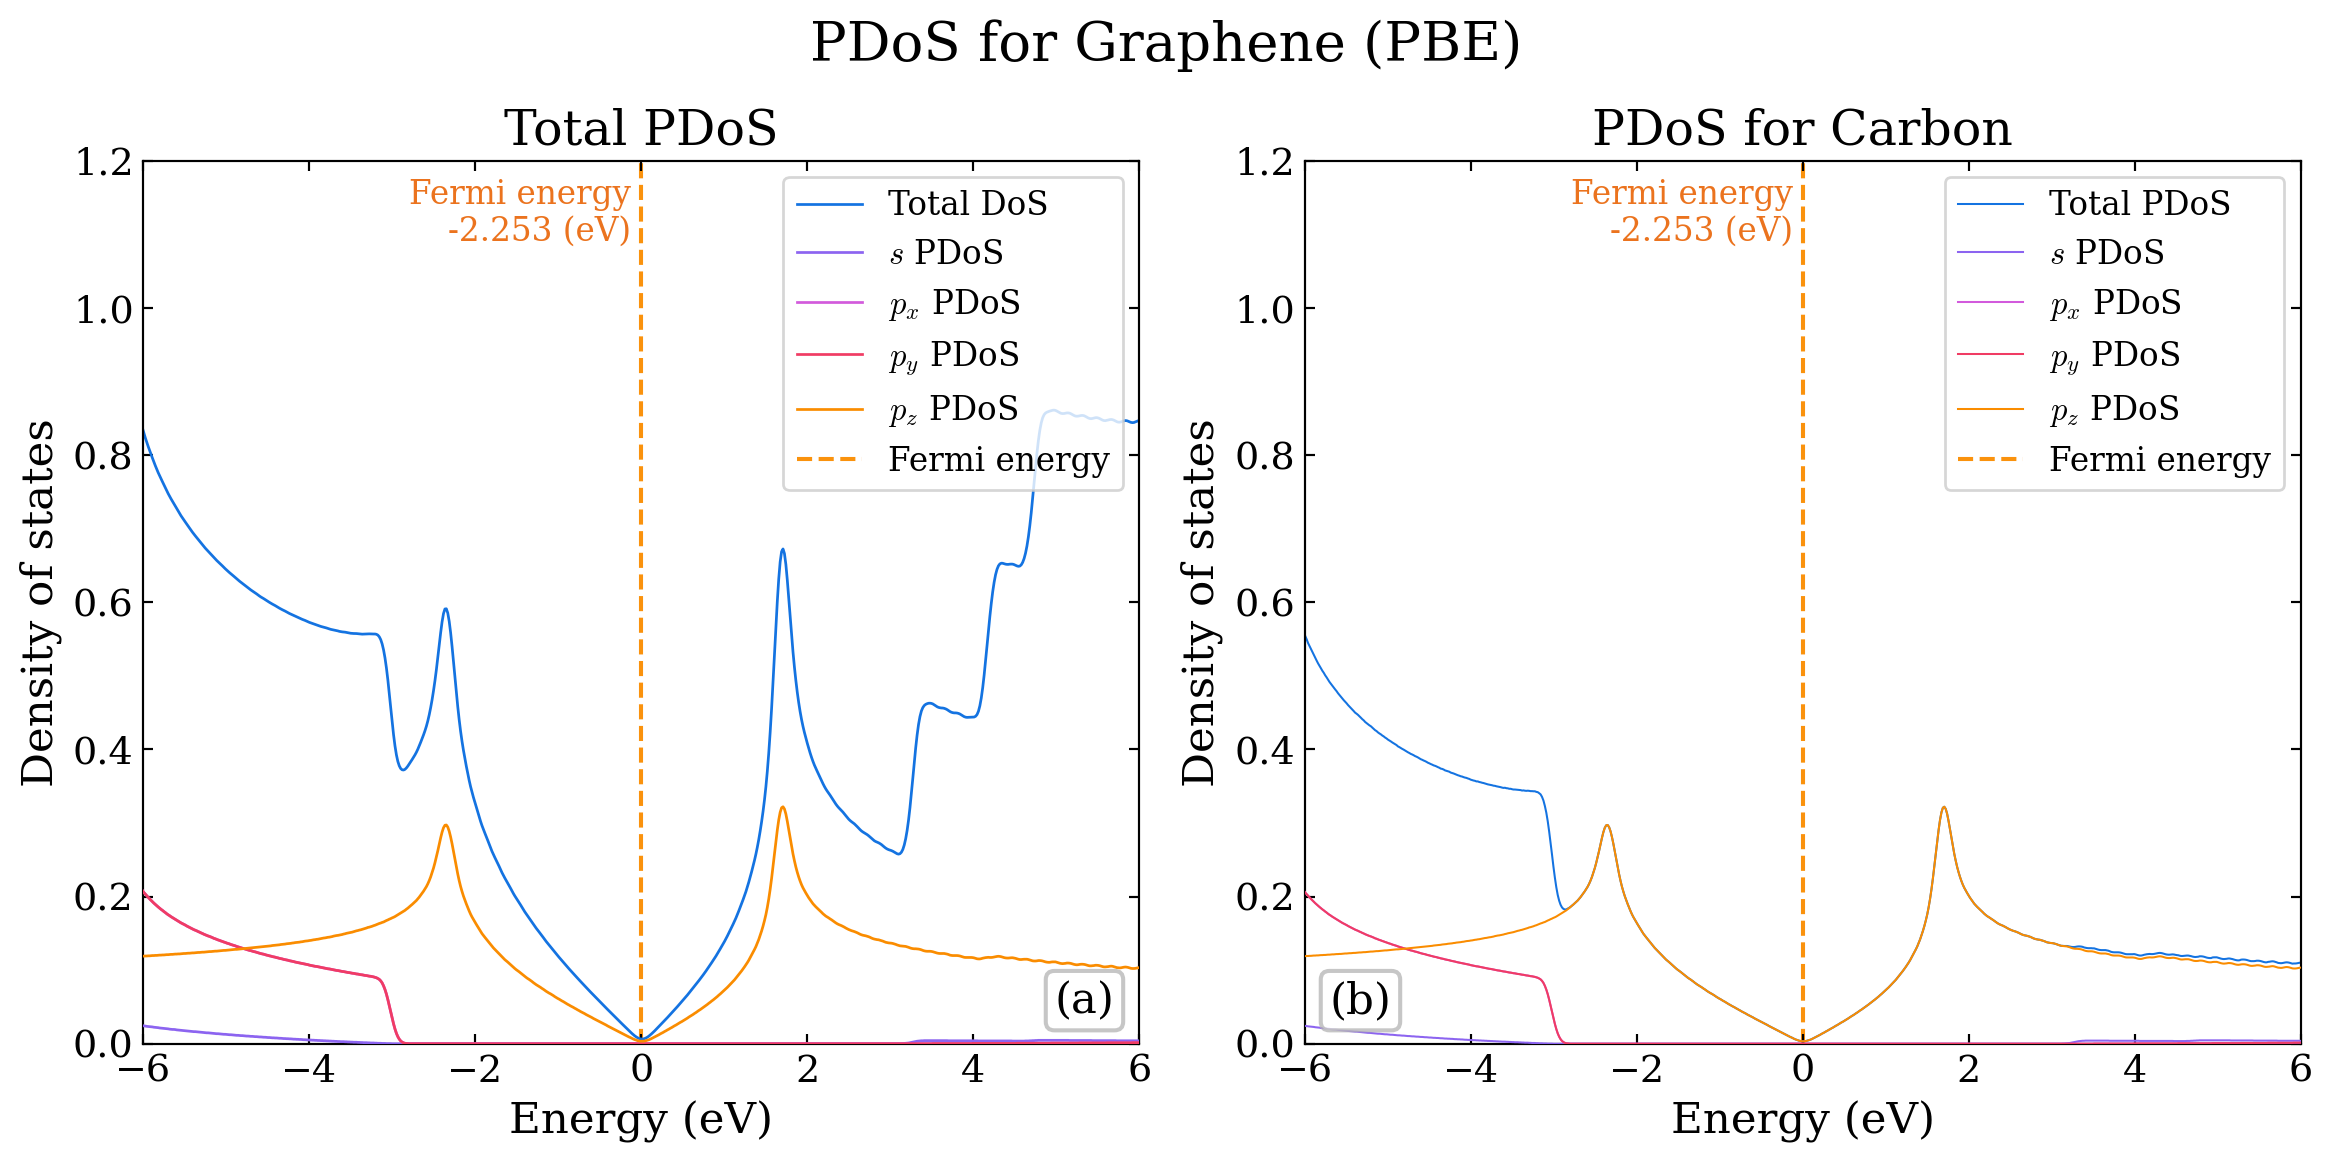
\includegraphics[width=0.8\textwidth]{PDoS/Graphene_pdos.png}
        \caption{Graphene PDoS}
    \end{figure}\end{column}
\end{columns}
\end{frame}

\section{Bilayers}

\subsection{Graphene-BC\texorpdfstring{$_\text{3}$}{3}: Hollow (PBE)}
\begin{frame}{\insertsection: \insertsubsection}
\begin{columns}
    \begin{column}{0.5\textwidth}\begin{figure}
        \includegraphics[width=0.5\textwidth]{Supercells/E_Graphene-BC3_Hollow.png}
        \caption{Graphene-BC$_\text{3}$ supercell}
    \end{figure}\end{column}
    \begin{column}{0.5\textwidth}
        \par \textbf{Bilayer: Graphene-BC$_\text{3}$}
        \par\quad LUMO band: -0.925600;
        \par\quad HOMO band: -0.928400;
        \par\quad Band gap: 0.002800.
    \end{column}
\end{columns}
\begin{columns}
    \begin{column}{0.45\textwidth}\begin{figure}
        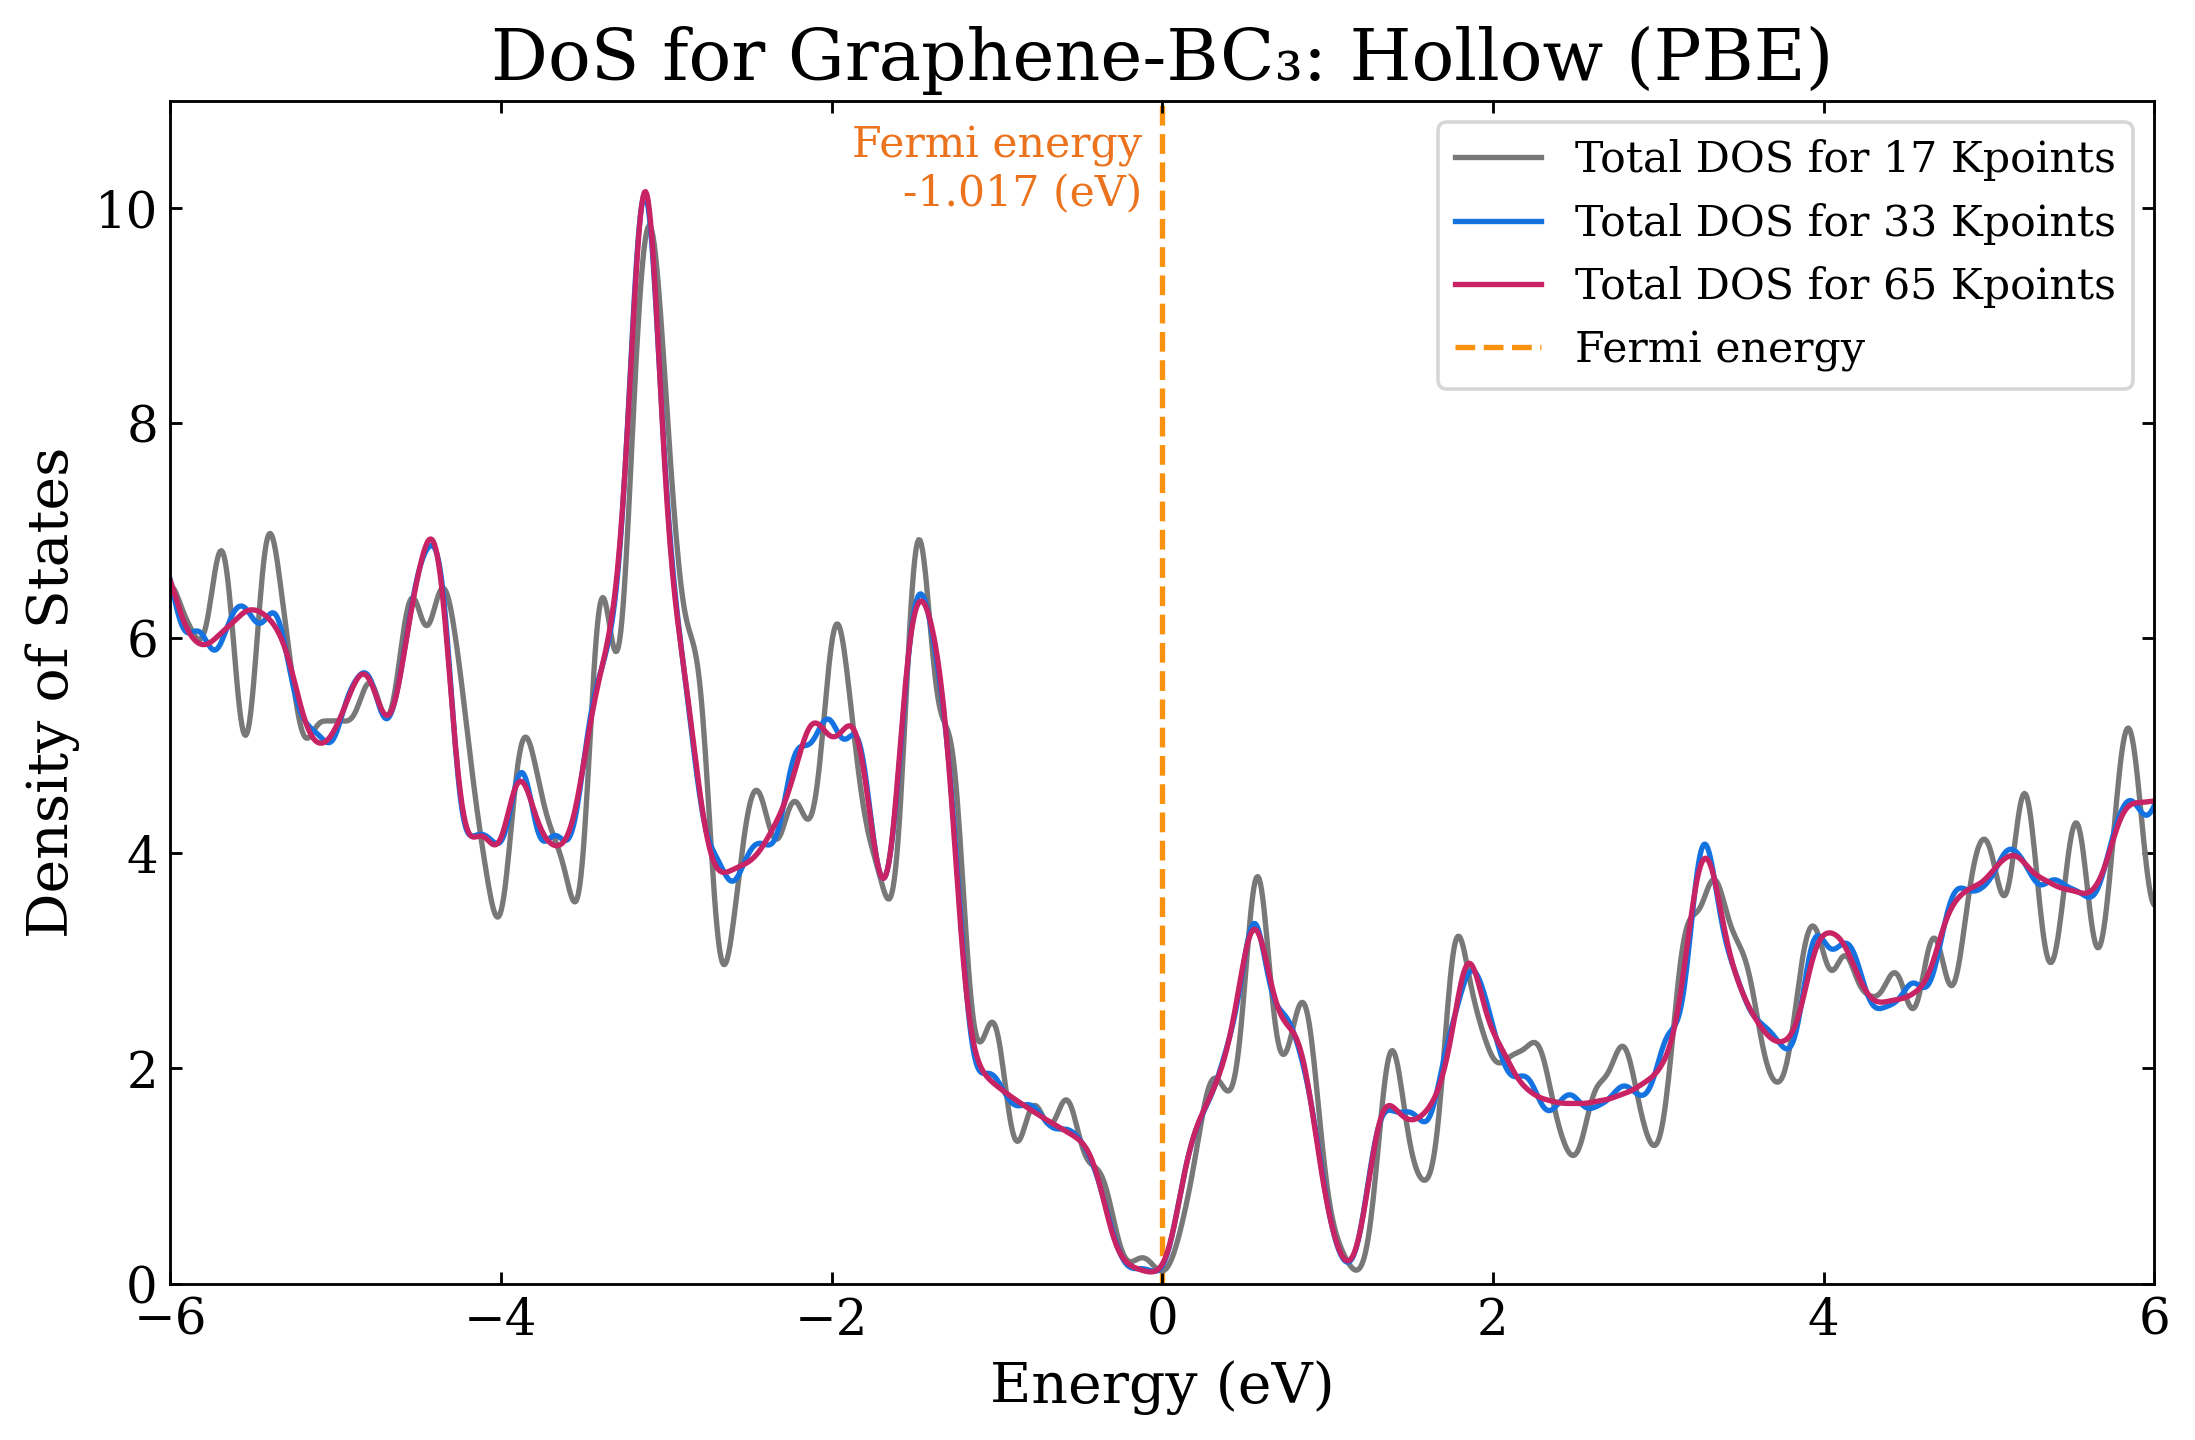
\includegraphics[width=1\textwidth]{PDoS/G-BC3_dos.png}
        \caption{Graphene-BC$_\text{3}$ DoS}
    \end{figure}\end{column}
    \begin{column}{0.55\textwidth}\begin{figure}
        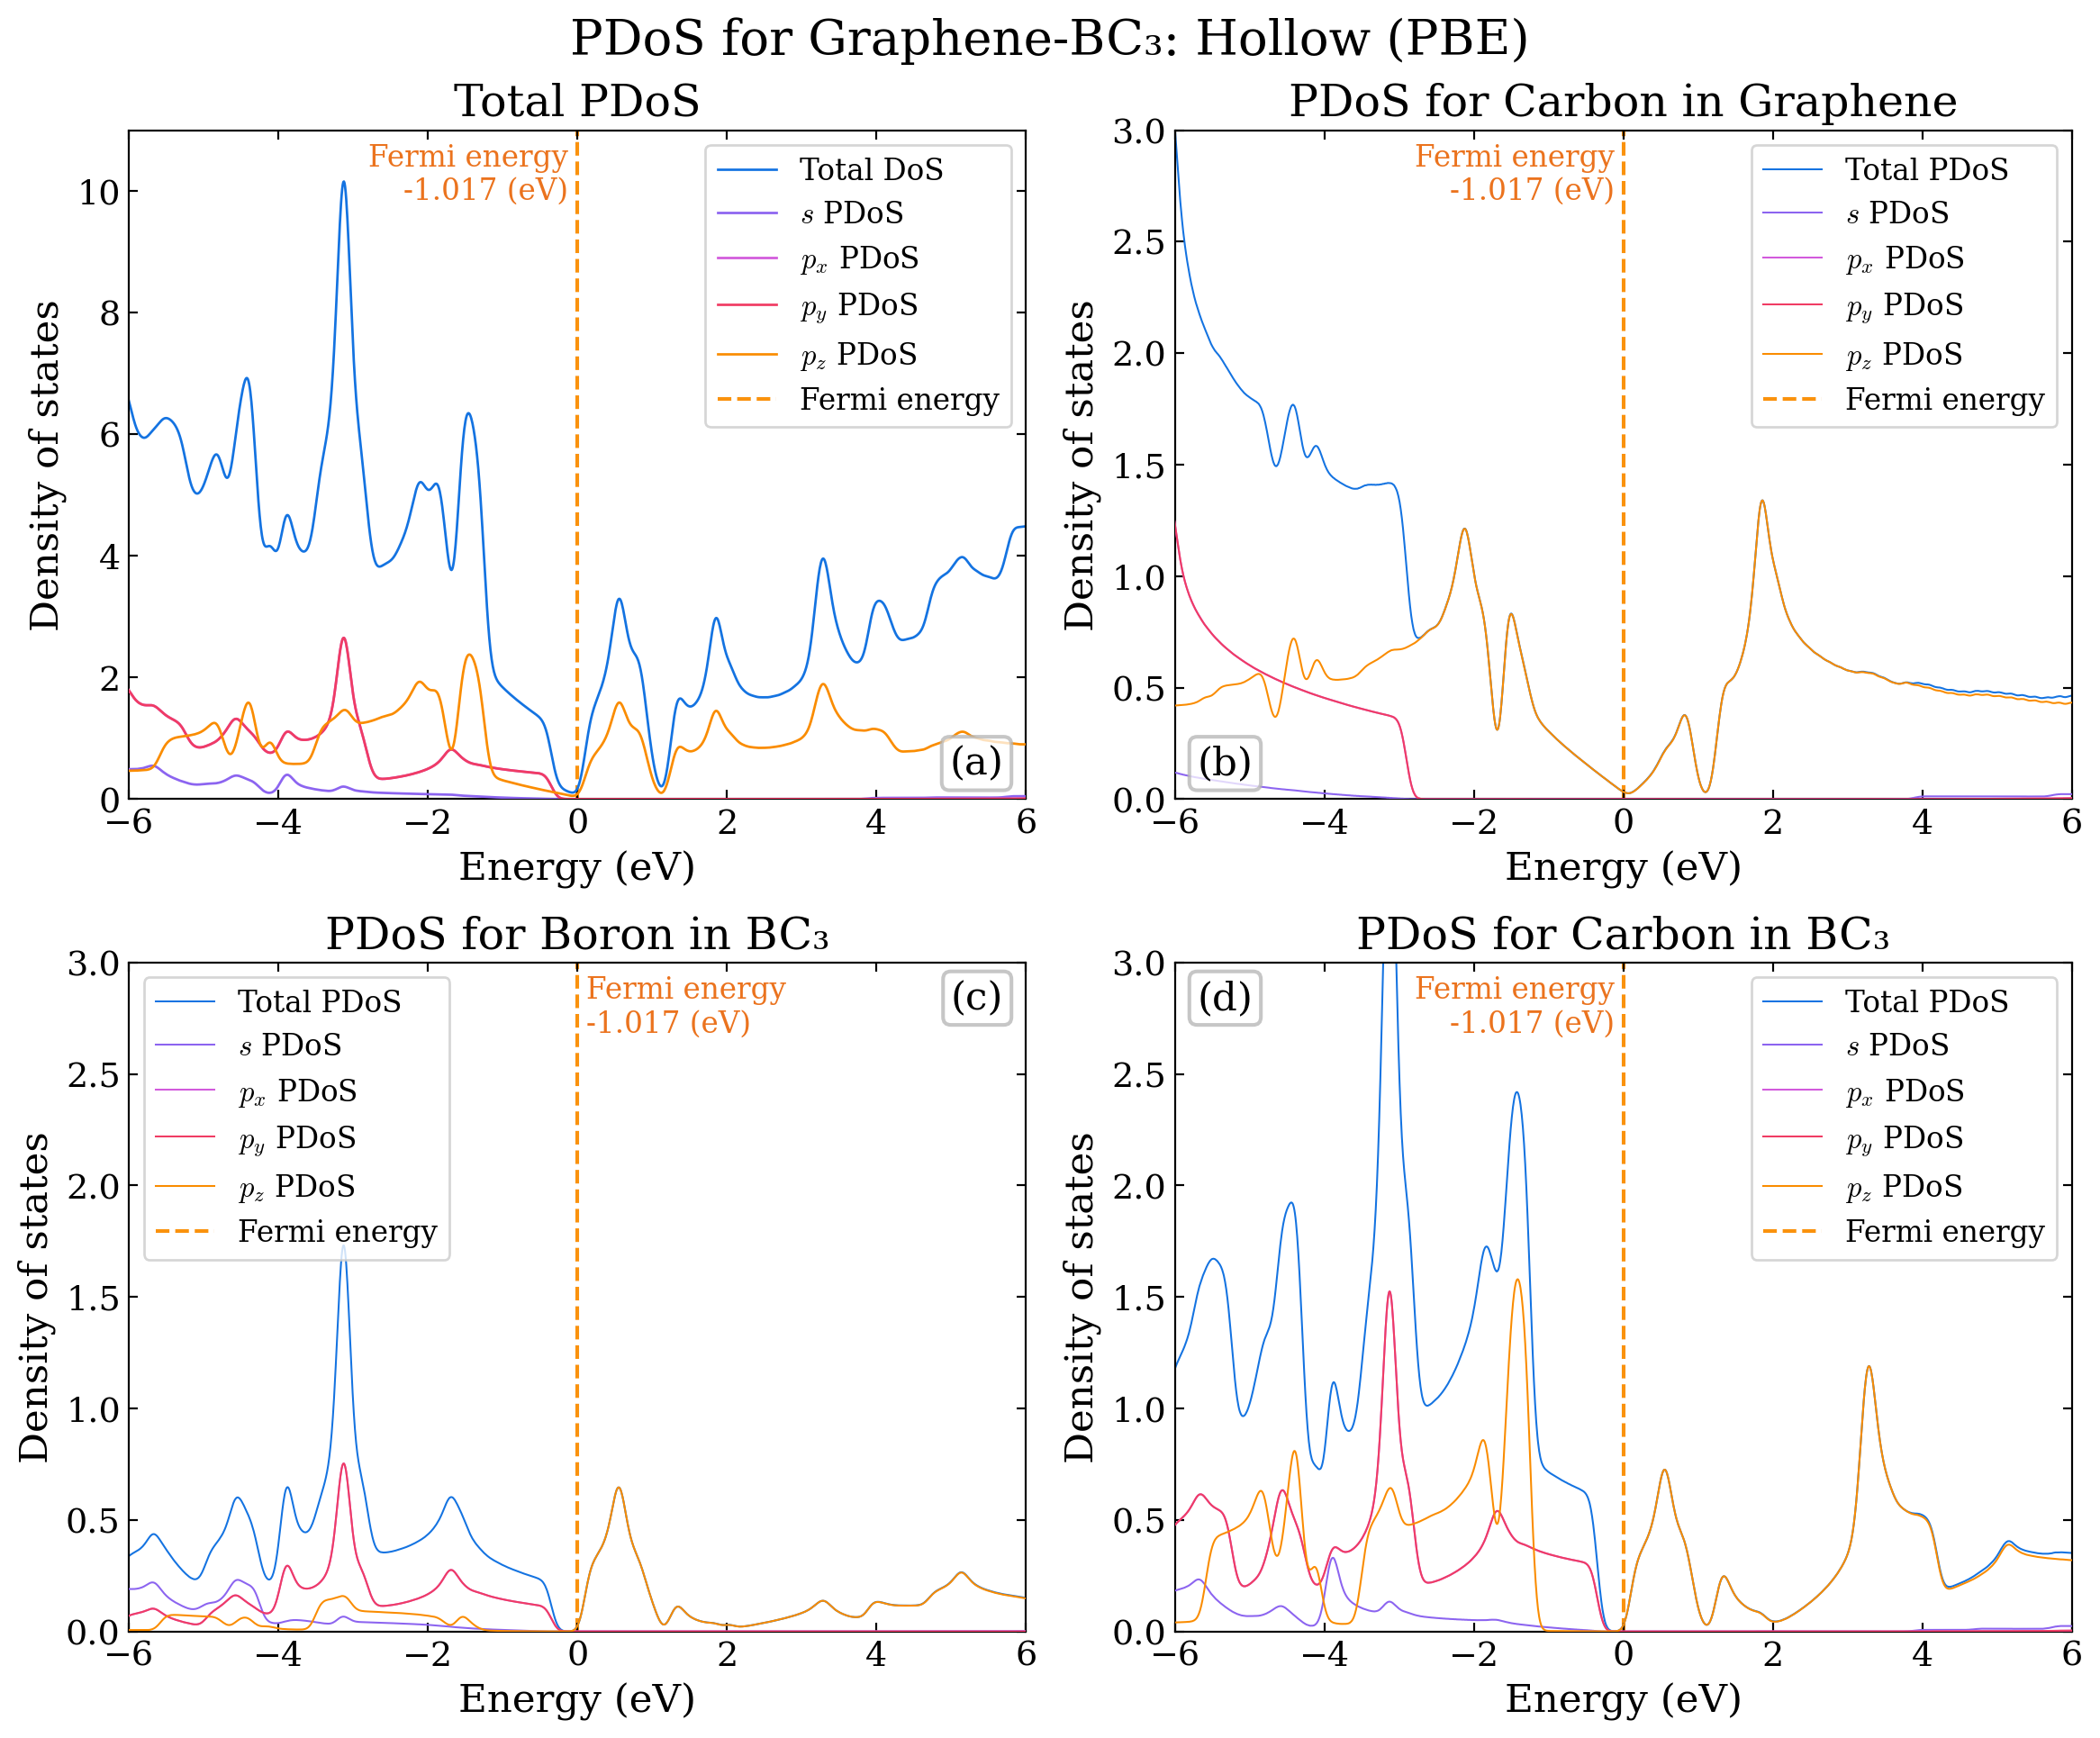
\includegraphics[width=0.8\textwidth]{PDoS/G-BC3_pdos.png}
        \caption{Graphene-BC$_\text{3}$ PDoS}
    \end{figure}\end{column}
\end{columns}
\end{frame}

\subsection{Graphene-Borophene: Top (PBE)}
\begin{frame}{\insertsection: \insertsubsection}
\begin{columns}
    \begin{column}{0.5\textwidth}\begin{figure}
        \includegraphics[width=0.5\textwidth]{Supercells/F_Graphene-Borophene_Top.png}
        \caption{Graphene-Borophene supercell}
    \end{figure}\end{column}
    \begin{column}{0.5\textwidth}
        \par \textbf{Bilayer: Graphene-Borophene}
        \par\quad LUMO band: -0.511000;
        \par\quad HOMO band: -0.310900;
        \par\quad Band gap: -0.200100.
    \end{column}
\end{columns}
\begin{columns}
    \begin{column}{0.45\textwidth}\begin{figure}
        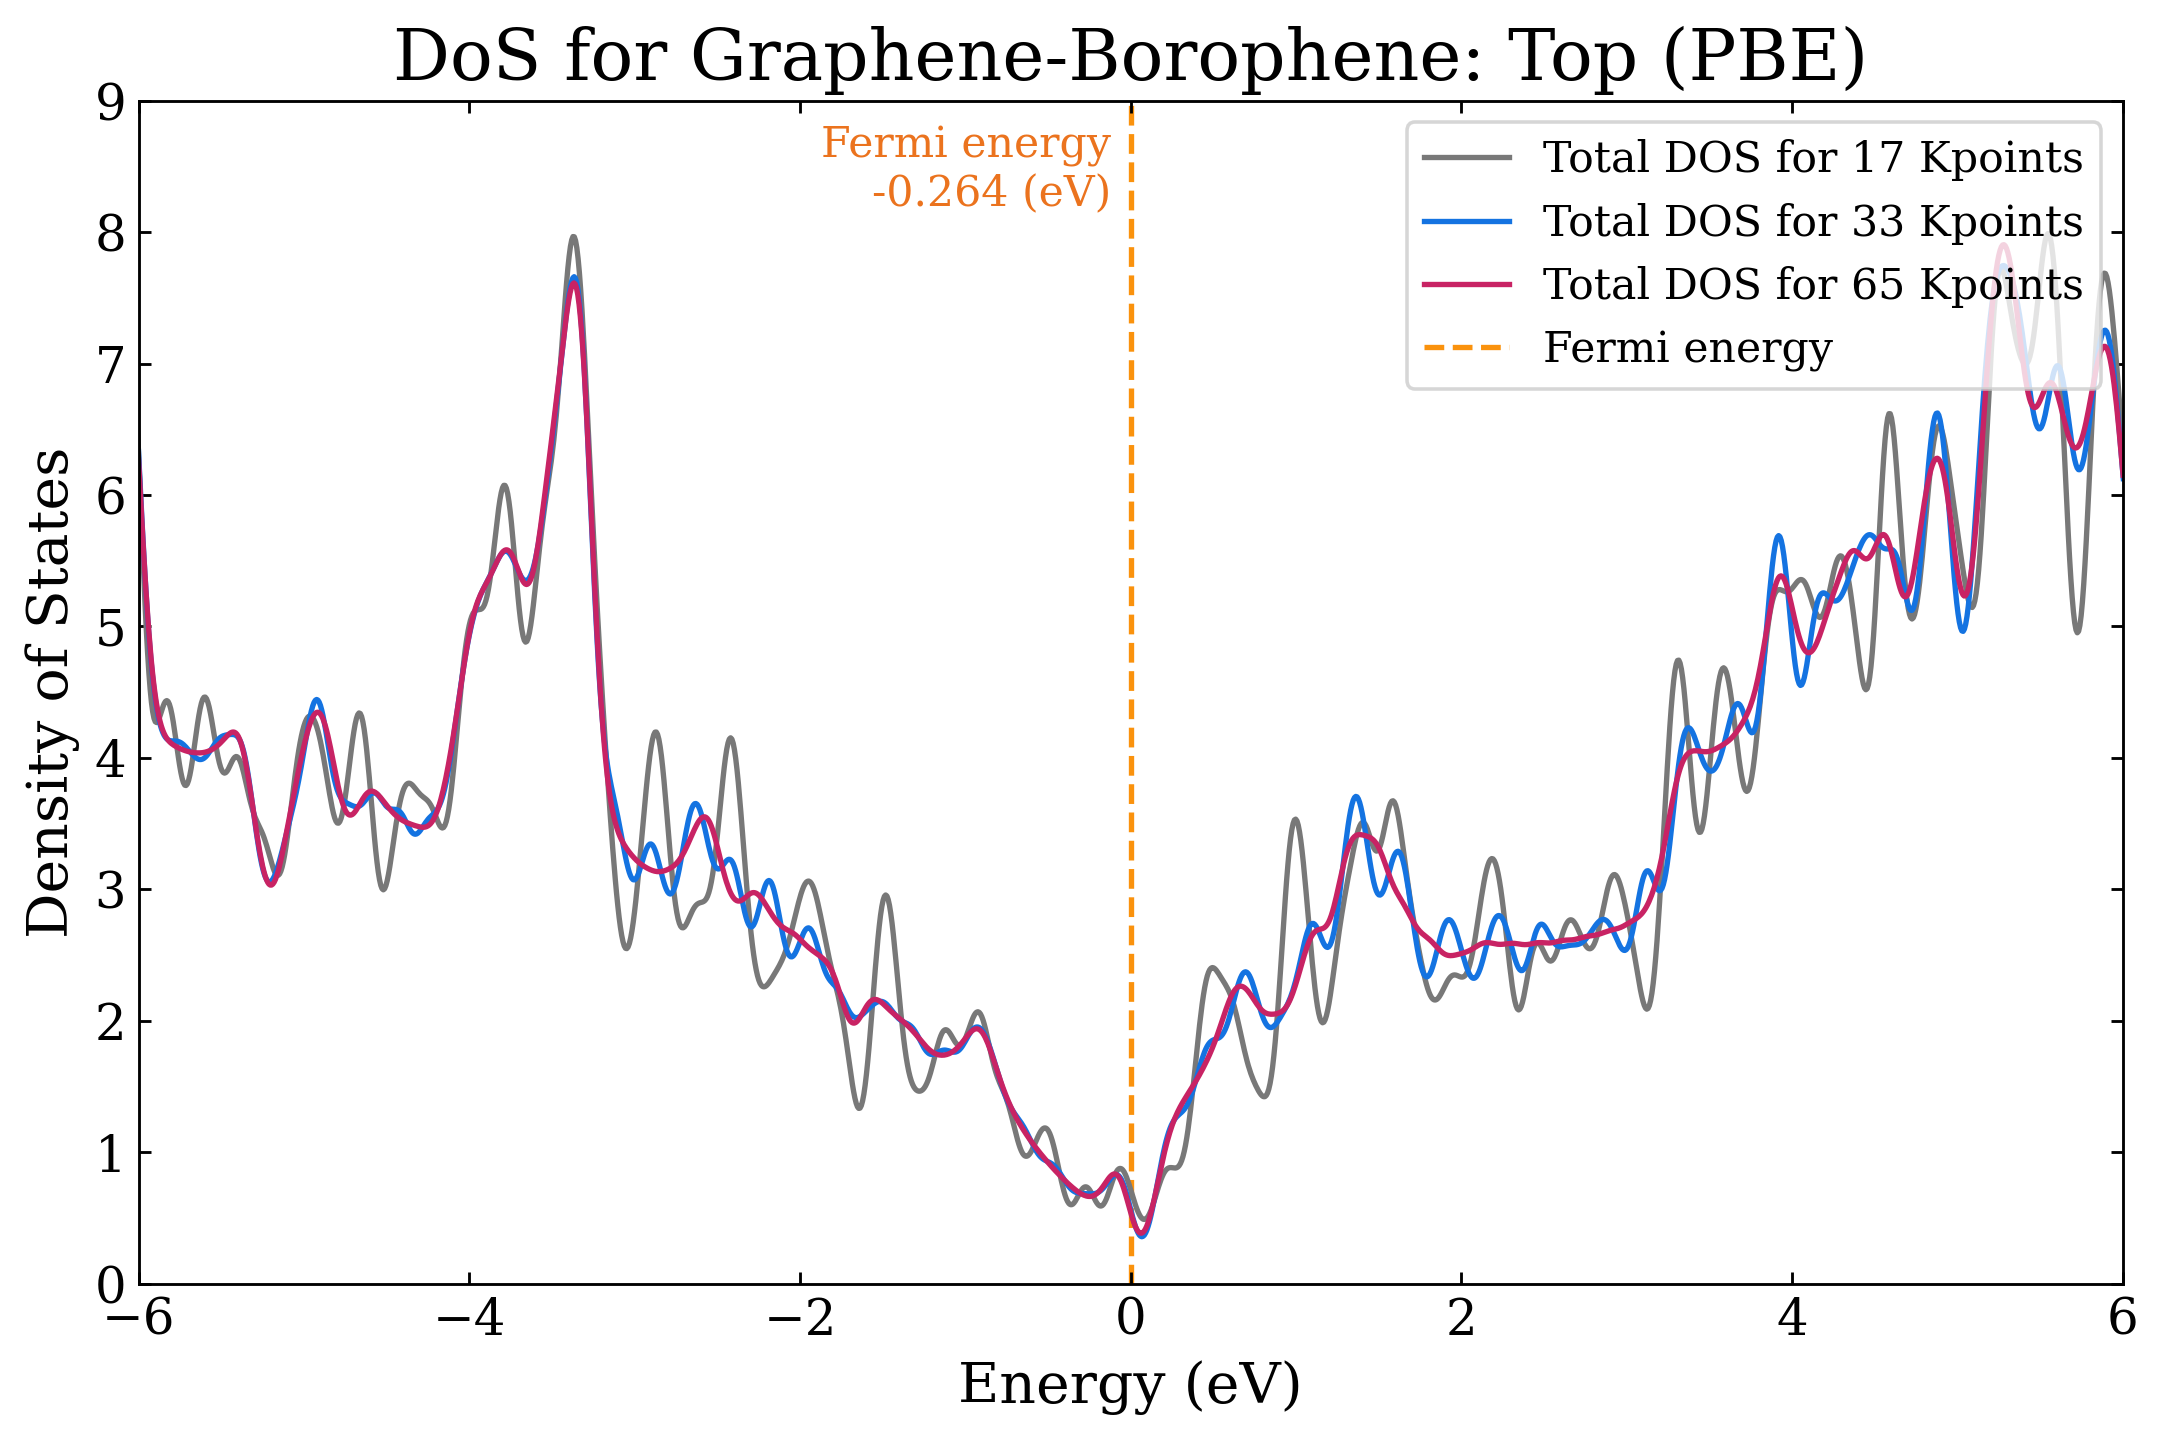
\includegraphics[width=1\textwidth]{PDoS/G-Borophene_dos.png}
        \caption{Graphene-Borophene DoS}
    \end{figure}\end{column}
    \begin{column}{0.55\textwidth}\begin{figure}
        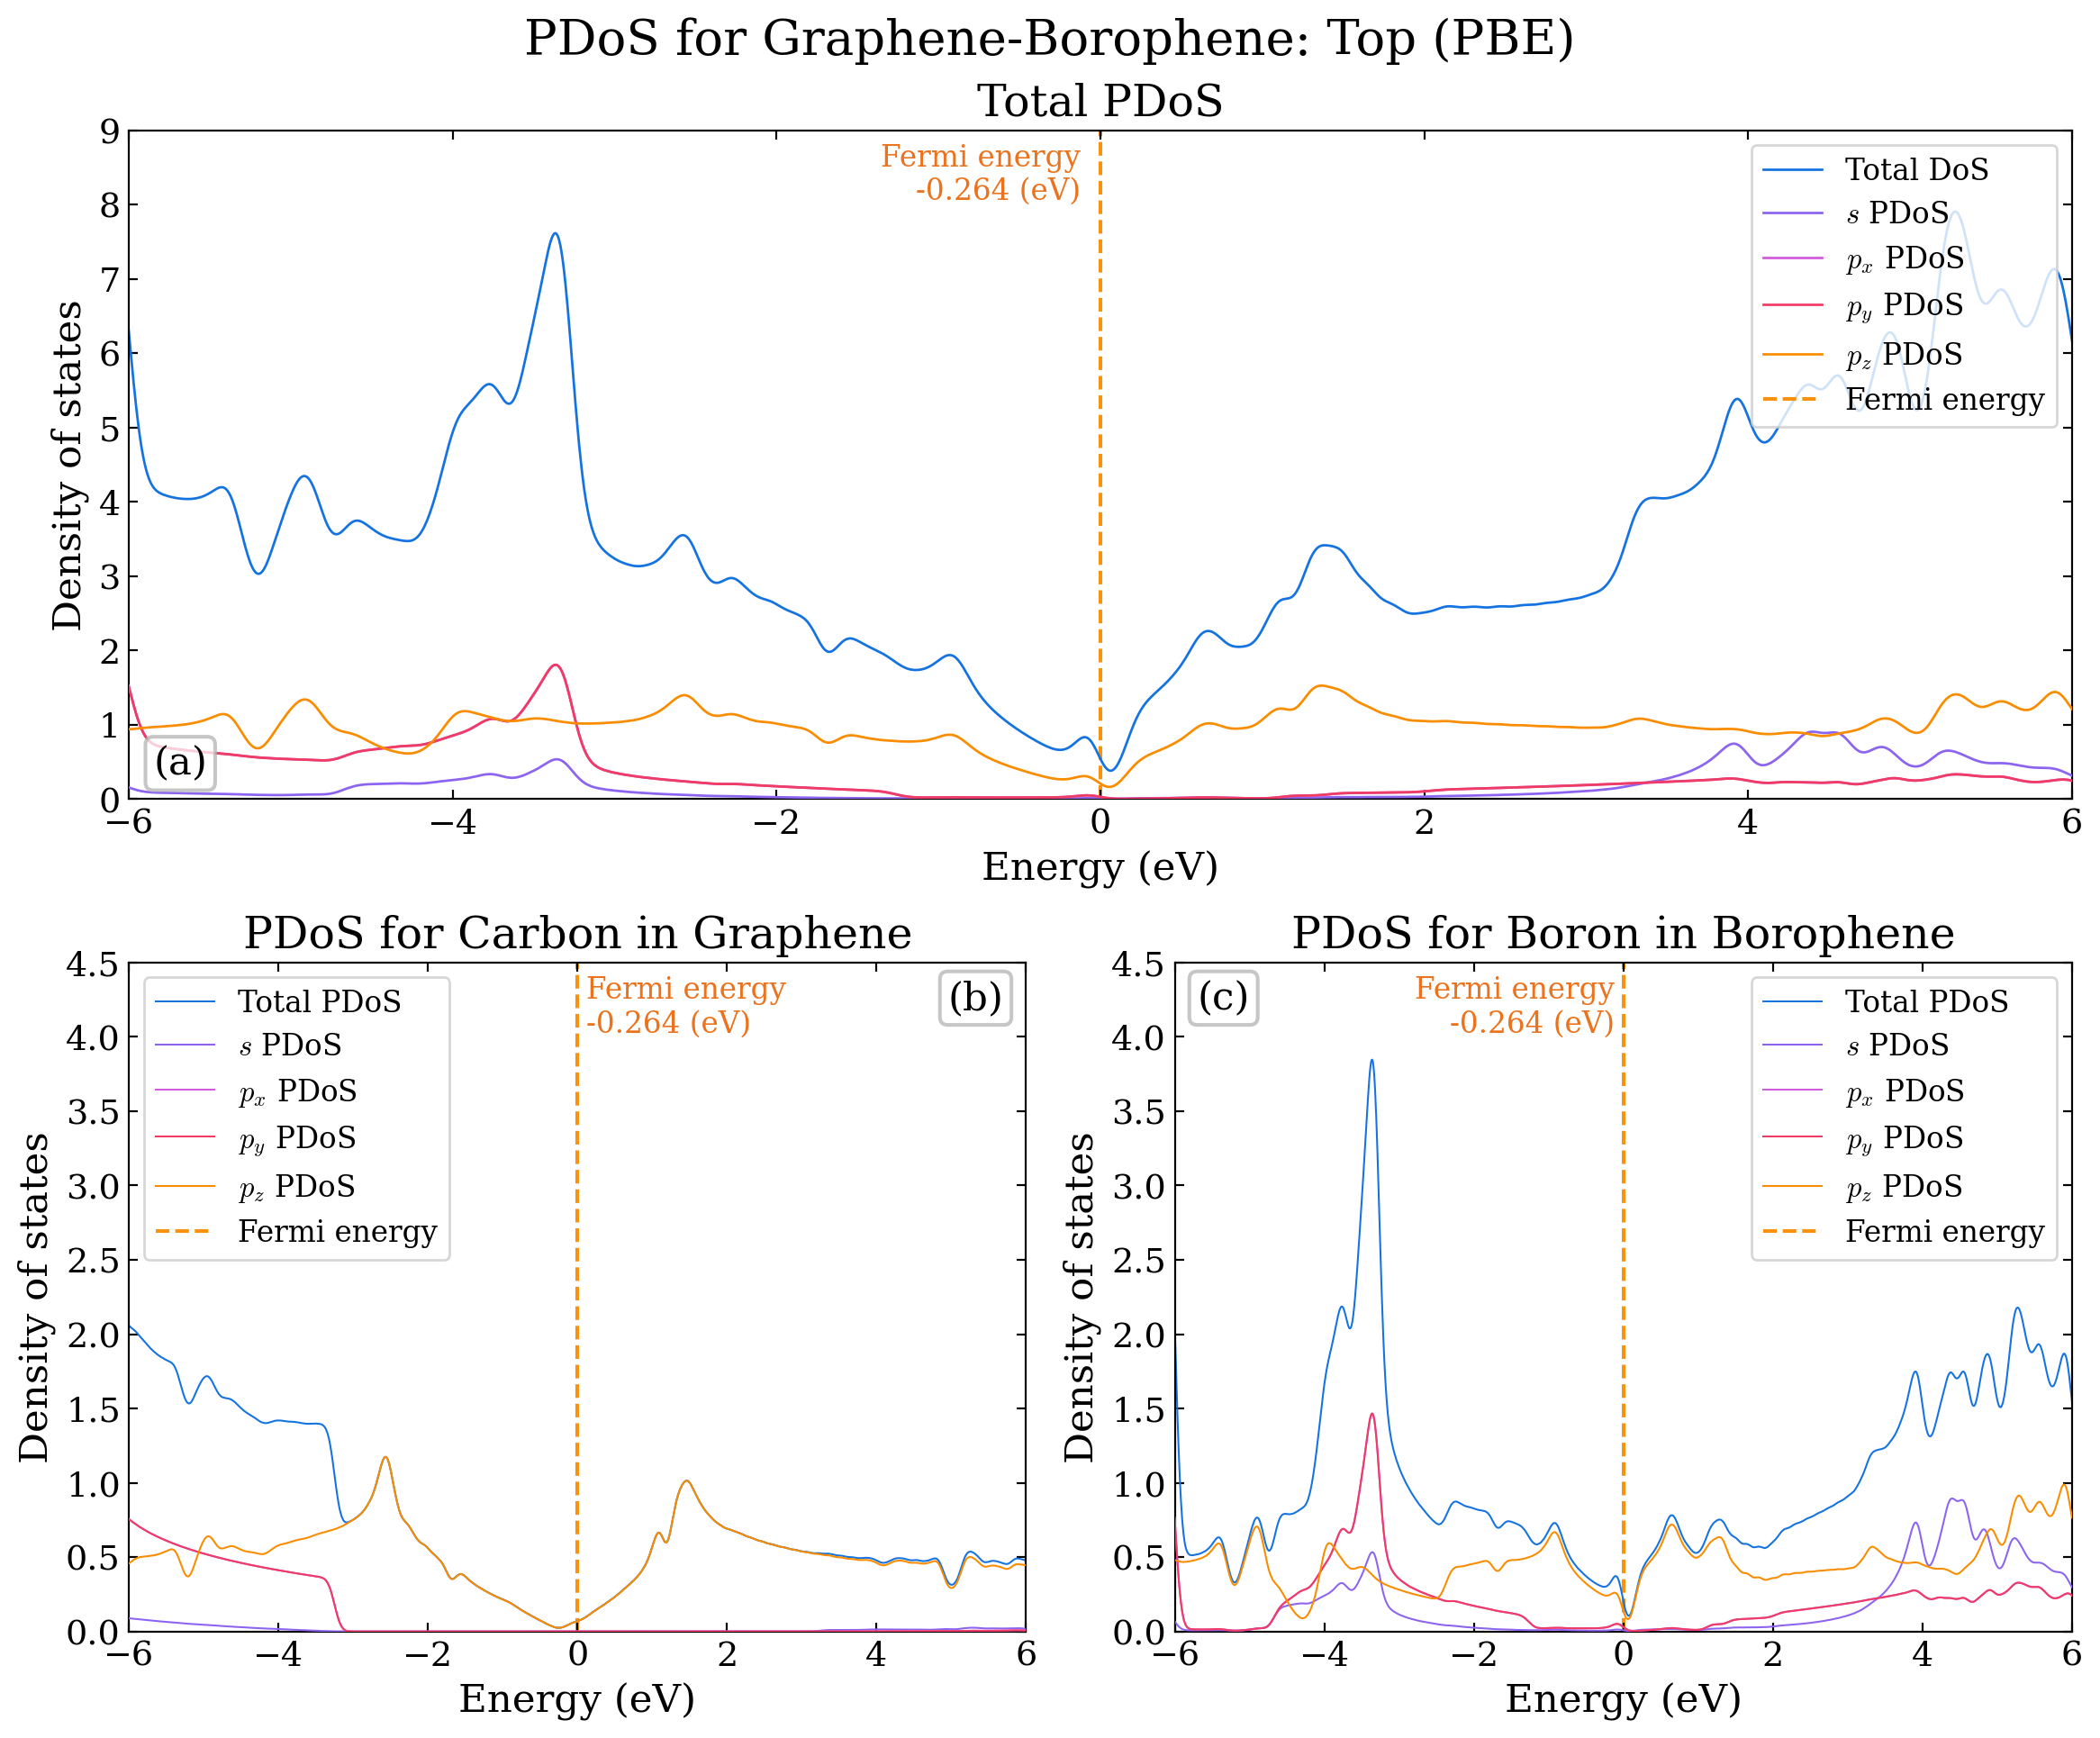
\includegraphics[width=0.8\textwidth]{PDoS/G-Borophene_pdos.png}
        \caption{Graphene-Borophene PDoS}
    \end{figure}\end{column}
\end{columns}
\end{frame}

\subsection{Graphene-B\texorpdfstring{$_\text{4}$}{4}C\texorpdfstring{$_\text{3}$}{3}: Top (PBE)}
\begin{frame}{\insertsection: \insertsubsection}
\begin{columns}
    \begin{column}{0.5\textwidth}\begin{figure}
        \includegraphics[width=0.5\textwidth]{Supercells/G_Graphene-B4C3_Top.png}
        \caption{Graphene-B$_\text{4}$C$_\text{3}$ supercell}
    \end{figure}\end{column}
    \begin{column}{0.5\textwidth}
        \par \textbf{Bilayer: Graphene-B$_\text{4}$C$_\text{3}$}
        \par\quad LUMO band: -0.314600;
        \par\quad HOMO band: -0.331300;
        \par\quad Band gap: 0.016700.
    \end{column}
\end{columns}
\begin{columns}
    \begin{column}{0.45\textwidth}\begin{figure}
        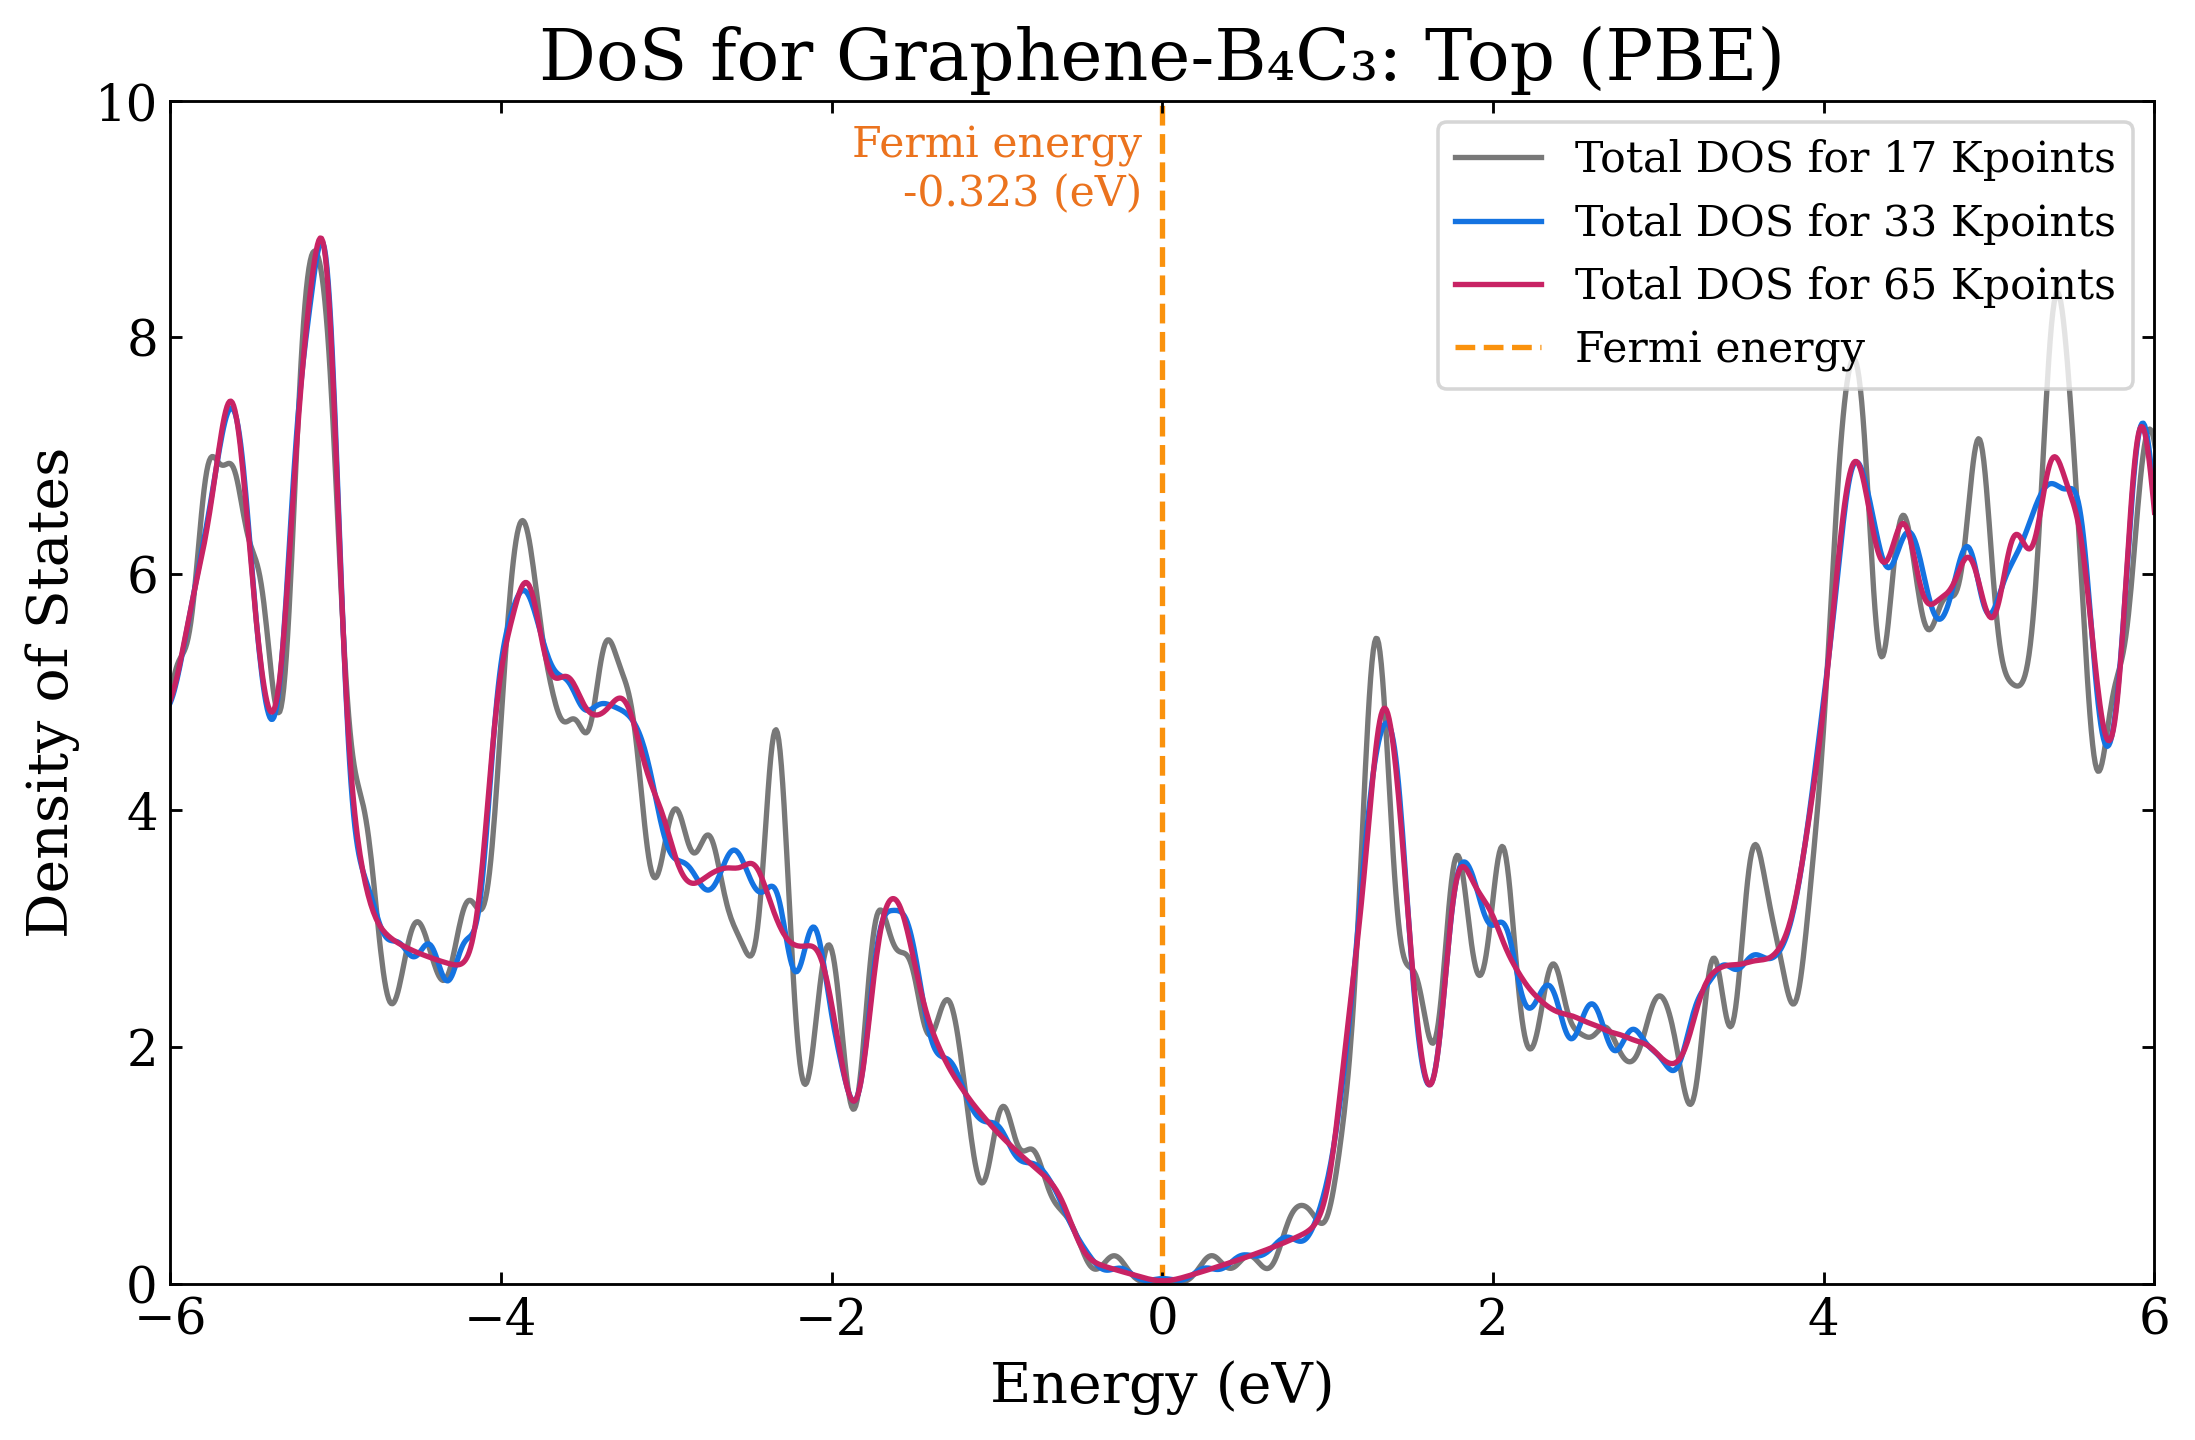
\includegraphics[width=1\textwidth]{PDoS/G-B4C3_dos.png}
        \caption{Graphene-B$_\text{4}$C$_\text{3}$ DoS}
    \end{figure}\end{column}
    \begin{column}{0.55\textwidth}\begin{figure}
        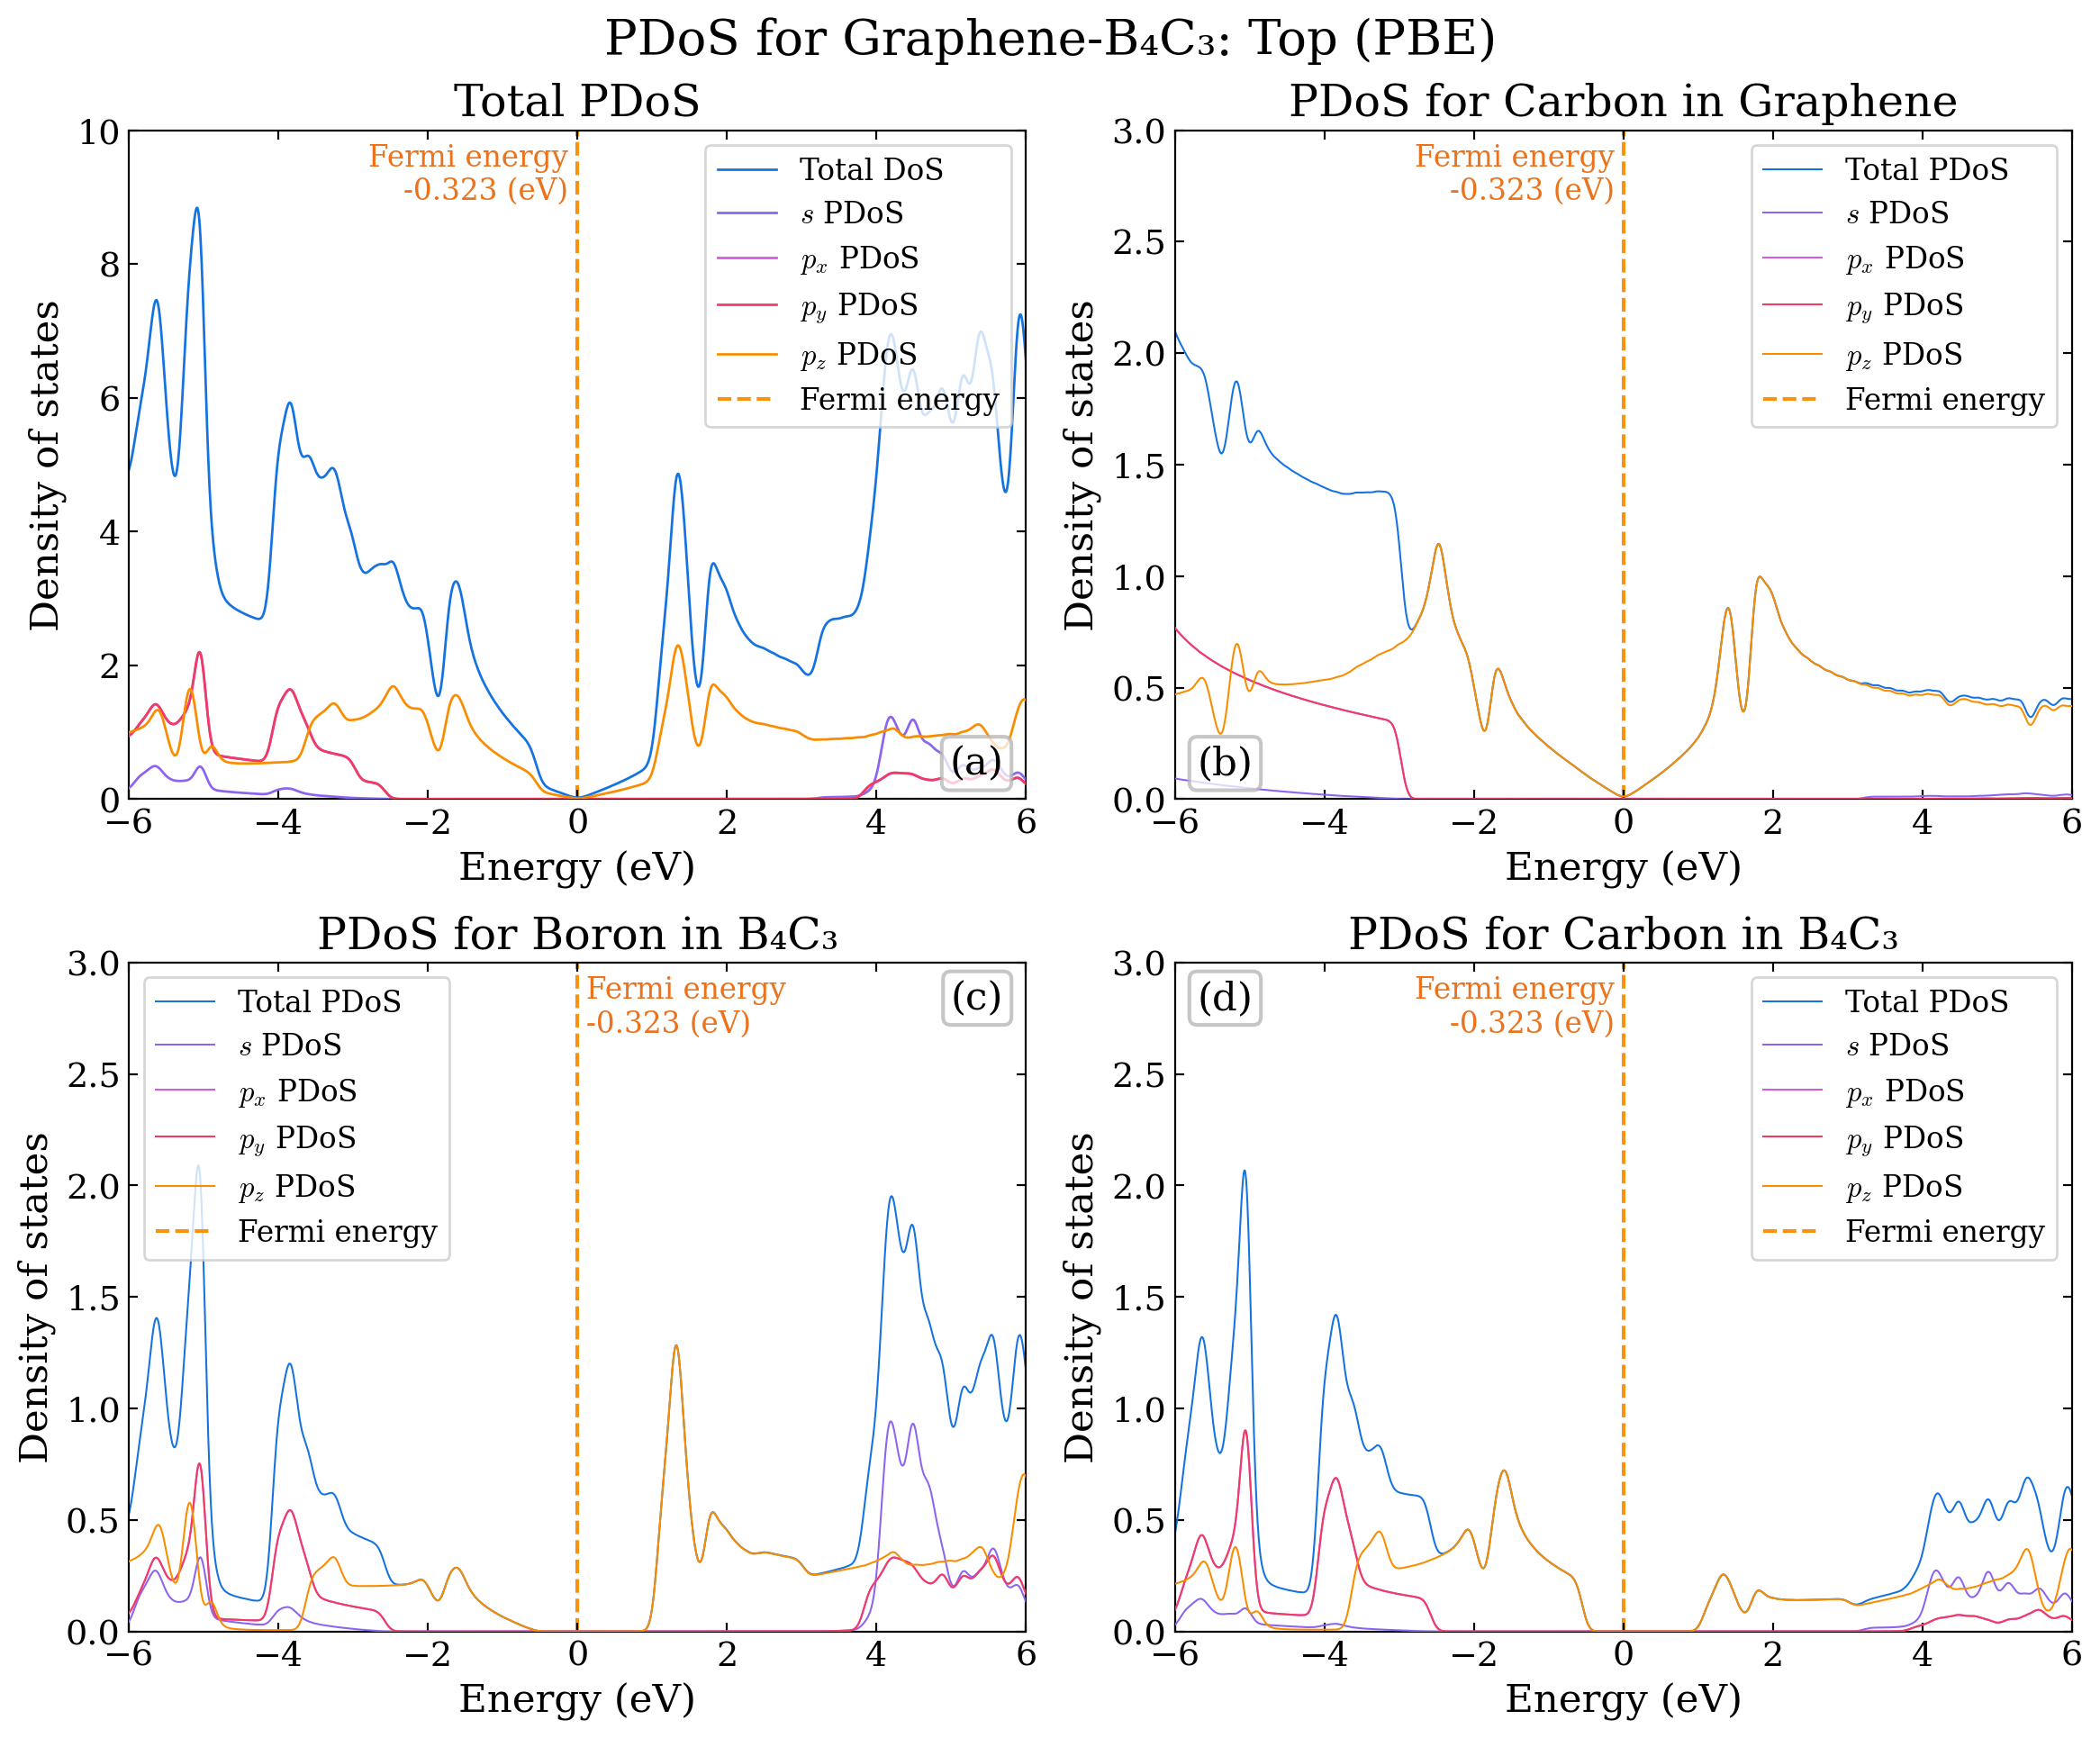
\includegraphics[width=0.8\textwidth]{PDoS/G-B4C3_pdos.png}
        \caption{Graphene-B$_\text{4}$C$_\text{3}$ PDoS}
    \end{figure}\end{column}
\end{columns}
\end{frame}

%% The End
\begin{frame}
    \begin{tikzpicture}[overlay, remember picture]
        % Background color box
        \node[fill=shallowTheme, rectangle, anchor=north, text width=\paperwidth, minimum height=40pt] at (current page.north) {};
        % Group logo
    \end{tikzpicture}
    \begin{tikzpicture}[overlay,remember picture]
        \node[anchor=north west]at(current page.north west){
\includegraphics[width=100pt]{Logo/USydLogo_White.png}};
    \end{tikzpicture}
    \Huge{\centerline{\textbf{Thank you}}}
\end{frame}

\end{document}
